\documentclass{beamer}
\usetheme{metropolis}
\usepackage{graphicx}
\usepackage{diagbox}
\usepackage{tcolorbox}
\title{Computer Logic and Digital Circuit Design (PHYS306/COSC330): Unit 3}
\author{Jordan Hanson}
\institute{Whittier College Department of Physics and Astronomy}

\begin{document}
\maketitle

\section{Summary}

\begin{frame}{Unit 3 Summary}
\alert{Functions of Combinatorial Logic} \\
\textbf{Reading:} 6-1 - 6-6 (Tuesday) \\
\textbf{Reading:} 6-7 - 6-11 (Thursday)
\begin{enumerate}
\item Half-Adders and Full-Adders
\begin{itemize}
\item Example from study guide
\item Propagation delays
\end{itemize}
\item Comparators
\begin{itemize}
\item The XNOR gate
\item Multi-bit comparators
\item Inequalities
\end{itemize}
\item Decoders/Encoders
\begin{itemize}
\item Binary to decimal circuits
\item Decimal to binary circuits
\end{itemize}
\end{enumerate}
\end{frame}

\section{Half-Adders and Full-Adders, Ripple-Carry}

\begin{frame}{Half-Adders and Full-Adders, Ripple-Carry}
\begin{figure}
\centering
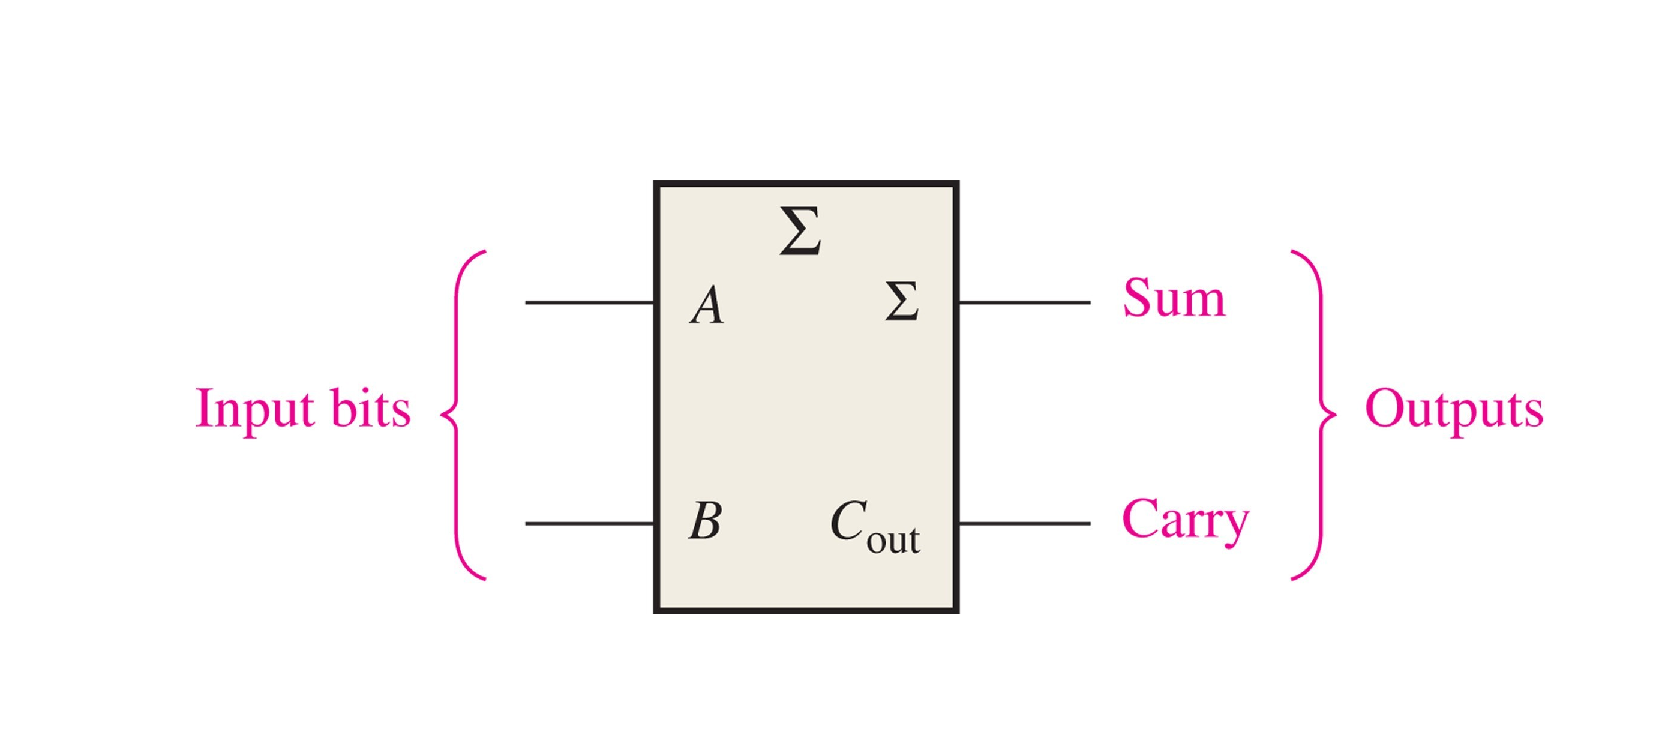
\includegraphics[width=0.9\textwidth]{figures/adder1.pdf}
\caption{\label{fig:add1} The desired inputs and outputs of the half-adder.  There is no carry-input.}
\end{figure}
\end{frame}

\begin{frame}{Half-Adders and Full-Adders, Ripple-Carry}
\begin{figure}
\centering
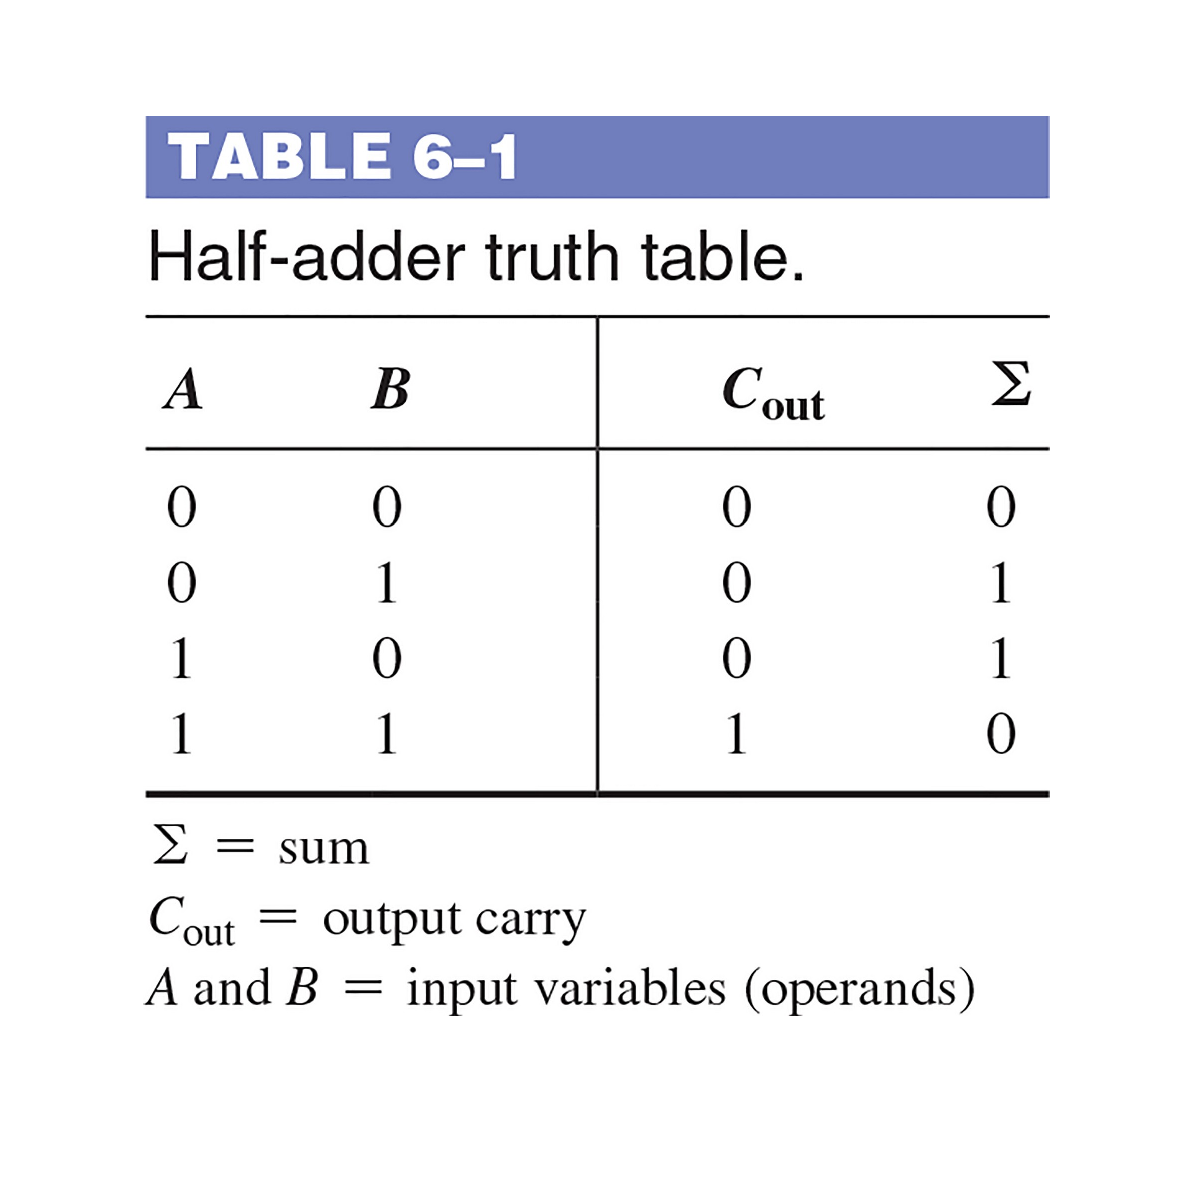
\includegraphics[width=0.5\textwidth]{figures/adder2.pdf}
\caption{\label{fig:add2} The truth table of the half-adder for 2-bits.  What gate action does this match?}
\end{figure}
\end{frame}

\begin{frame}{Half-Adders and Full-Adders, Ripple-Carry}
\begin{figure}
\centering
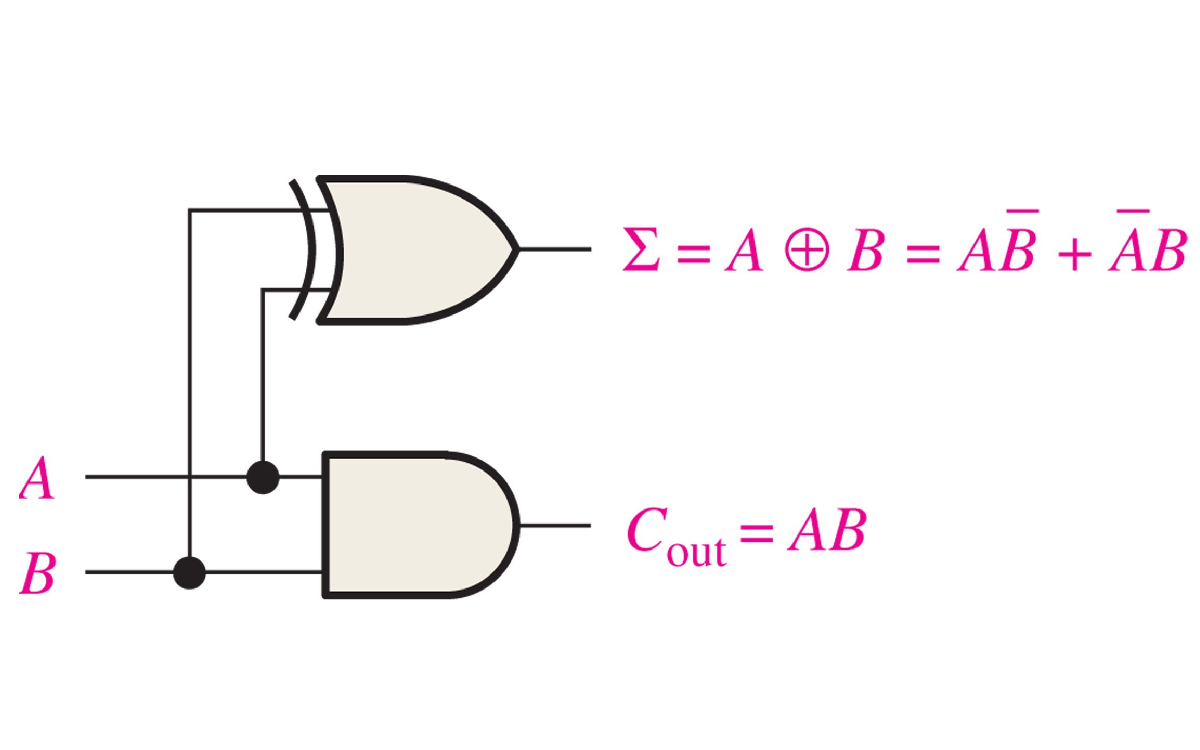
\includegraphics[width=0.7\textwidth]{figures/adder3.pdf}
\caption{\label{fig:add3} The logic function circuit diagram for the half-adder.}
\end{figure}
\end{frame}

\begin{frame}{Half-Adders and Full-Adders, Ripple-Carry}
\begin{figure}
\centering
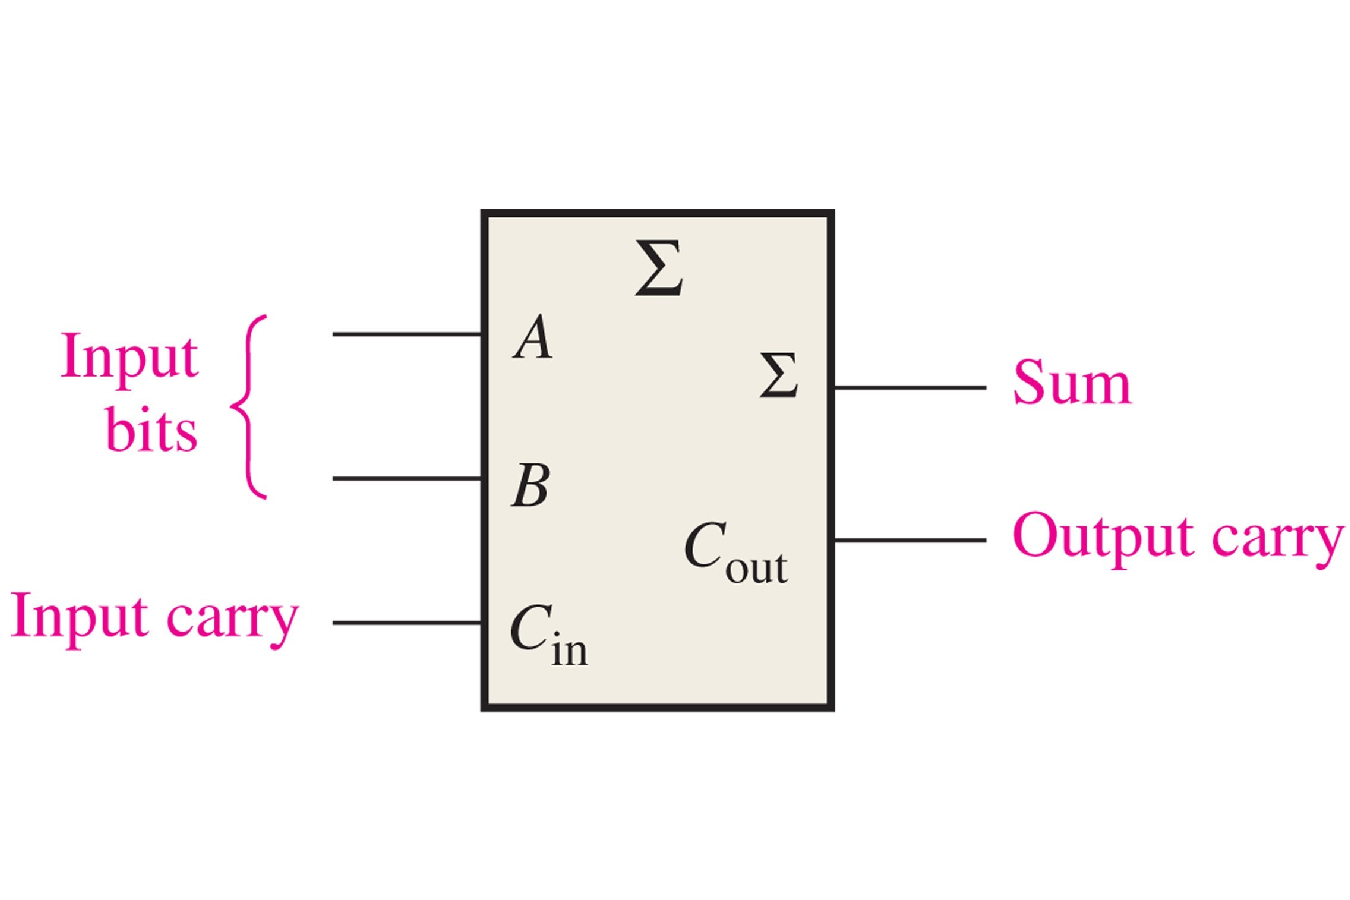
\includegraphics[width=0.7\textwidth]{figures/adder4.pdf}
\caption{\label{fig:add4} The desired inputs and outputs for the full-adder, with carry-input and carry-output.}
\end{figure}
\end{frame}

\begin{frame}{Half-Adders and Full-Adders, Ripple-Carry}
\begin{figure}
\centering
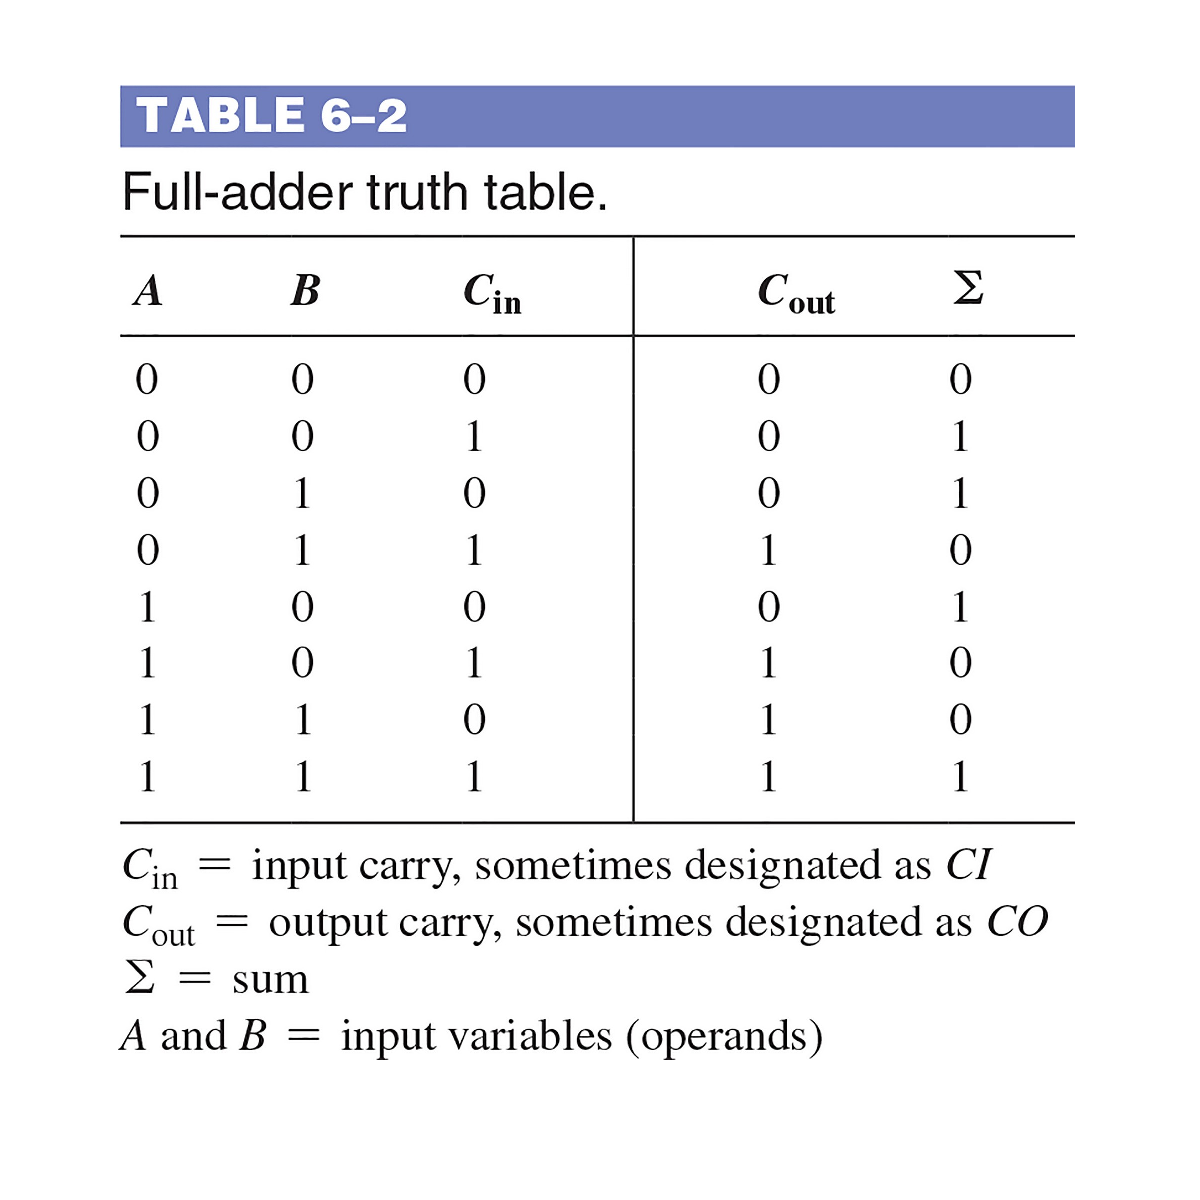
\includegraphics[width=0.5\textwidth]{figures/adder5.pdf}
\caption{\label{fig:add5} The truth table for the full-adder is more complex due to the increased number of inputs.}
\end{figure}
\end{frame}

\begin{frame}{Half-Adders and Full-Adders, Ripple-Carry}
\begin{figure}
\centering
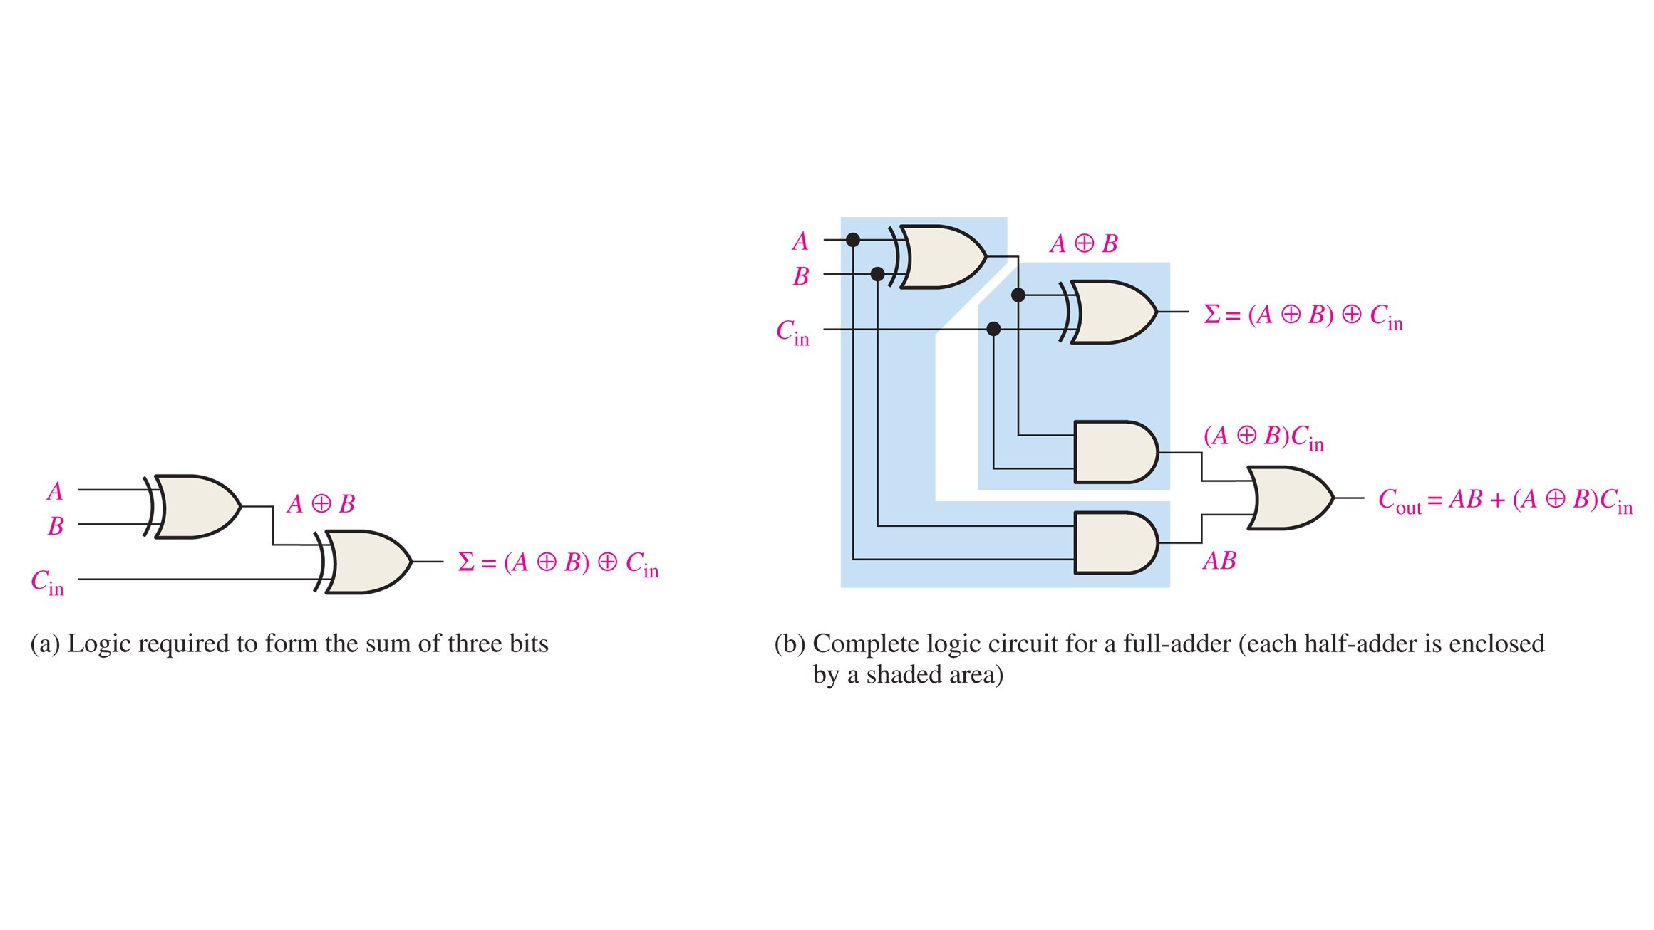
\includegraphics[width=0.9\textwidth]{figures/adder6.pdf}
\caption{\label{fig:add6} Circuit diagrams for the half-adder (left) and full-adder (right).}
\end{figure}
\end{frame}

\begin{frame}{Half-Adders and Full-Adders, Ripple-Carry}
\begin{figure}
\centering
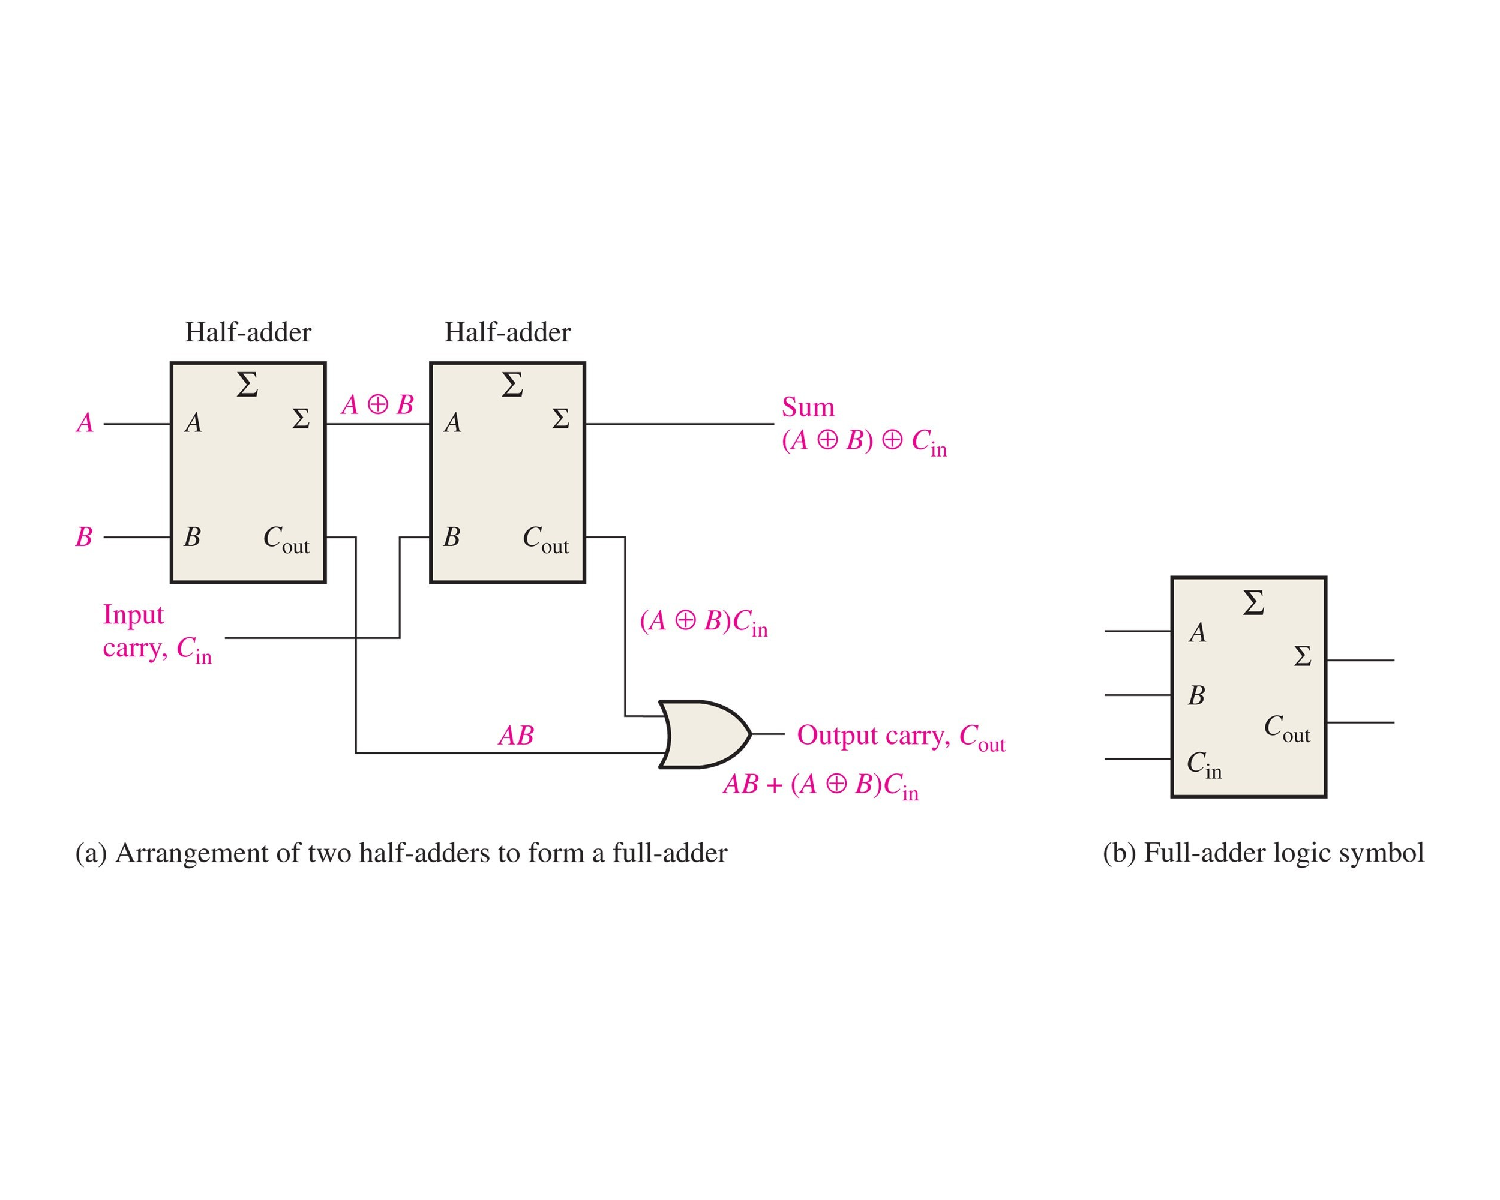
\includegraphics[width=0.7\textwidth]{figures/adder7.pdf}
\caption{\label{fig:add7} Two half-adders to form a full-adder.}
\end{figure}
\end{frame}

\begin{frame}{Half-Adders and Full-Adders, Ripple-Carry}
\begin{figure}
\centering
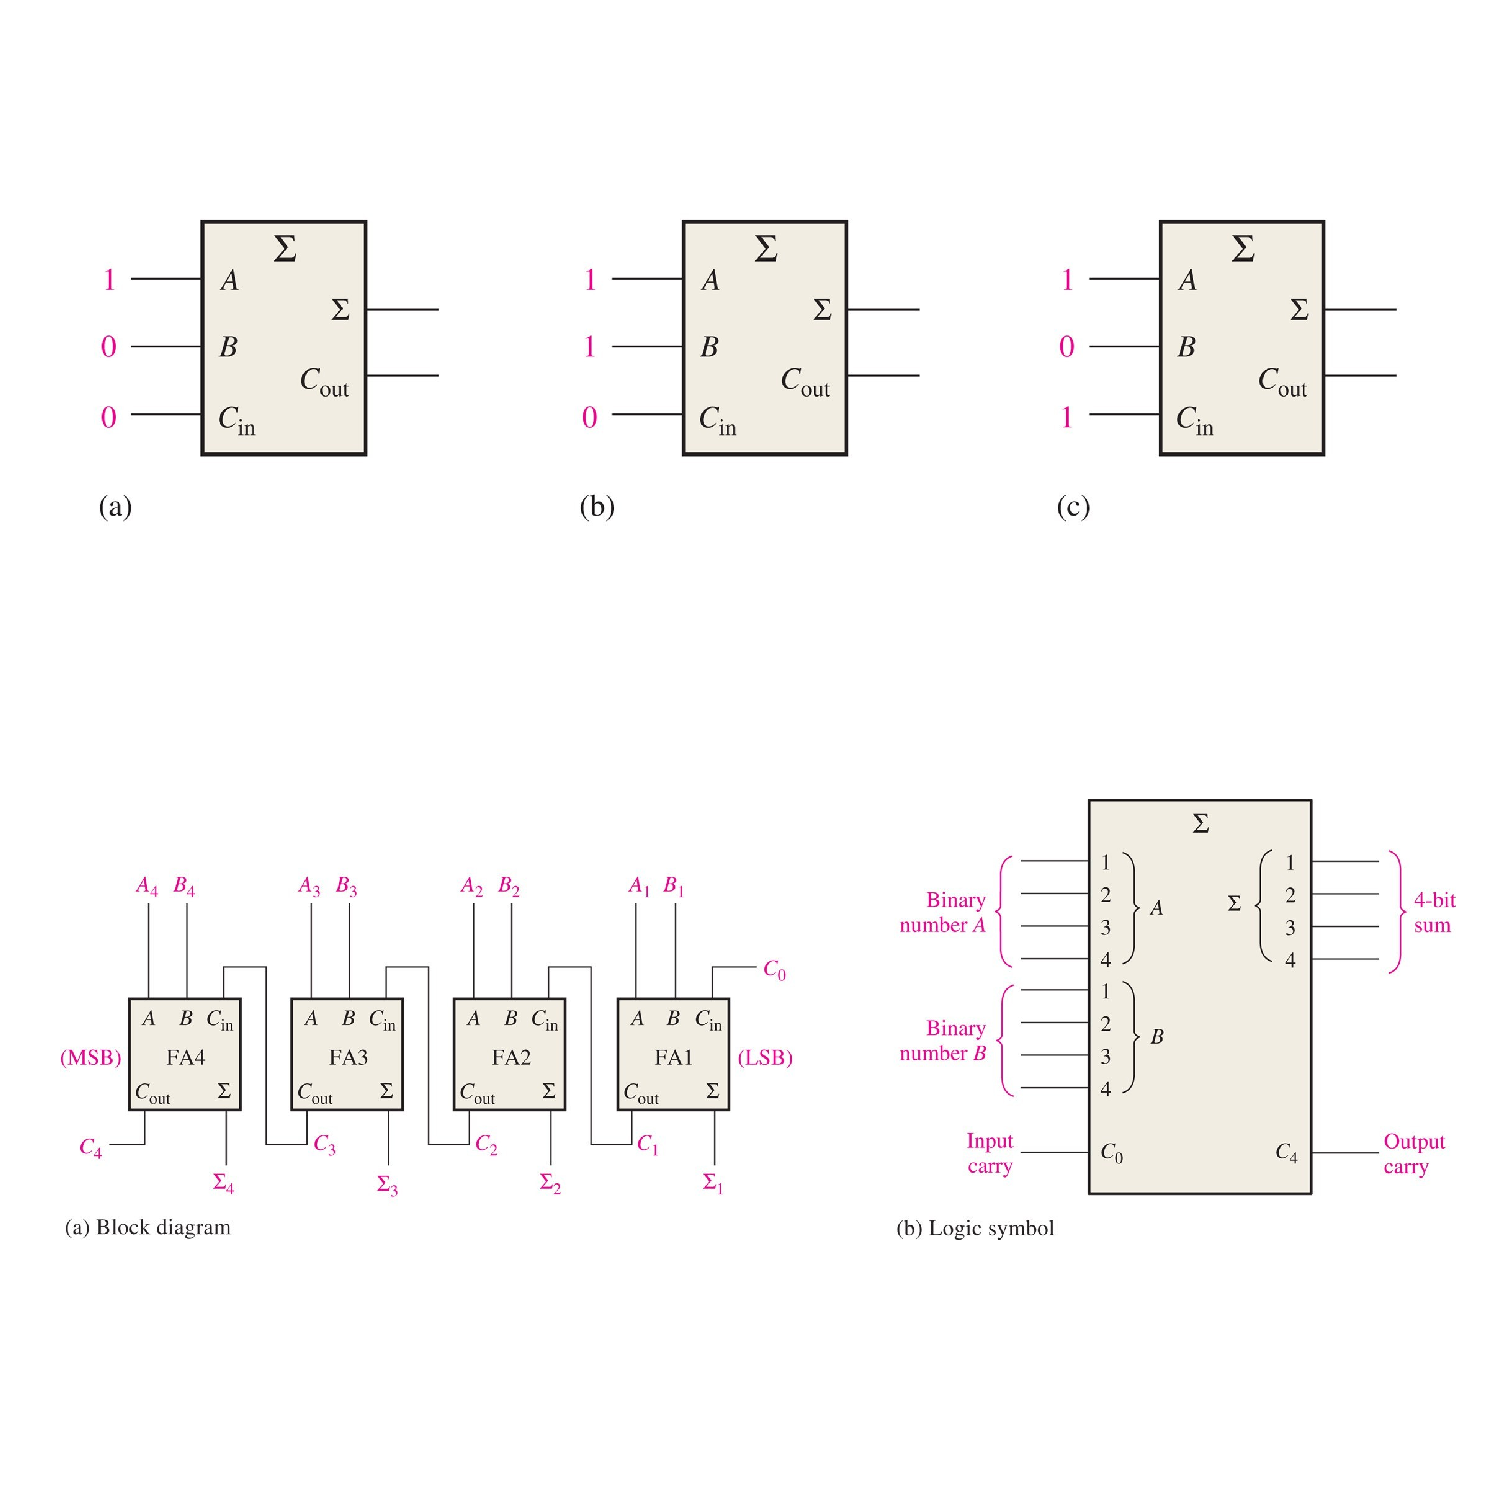
\includegraphics[width=0.5\textwidth]{figures/adder8.pdf}
\caption{\label{fig:add8} Four FA (full-adders) to add bits to the numbers being added.}
\end{figure}
\end{frame}

\begin{frame}{Half-Adders and Full-Adders, Ripple-Carry}
\begin{figure}
\centering
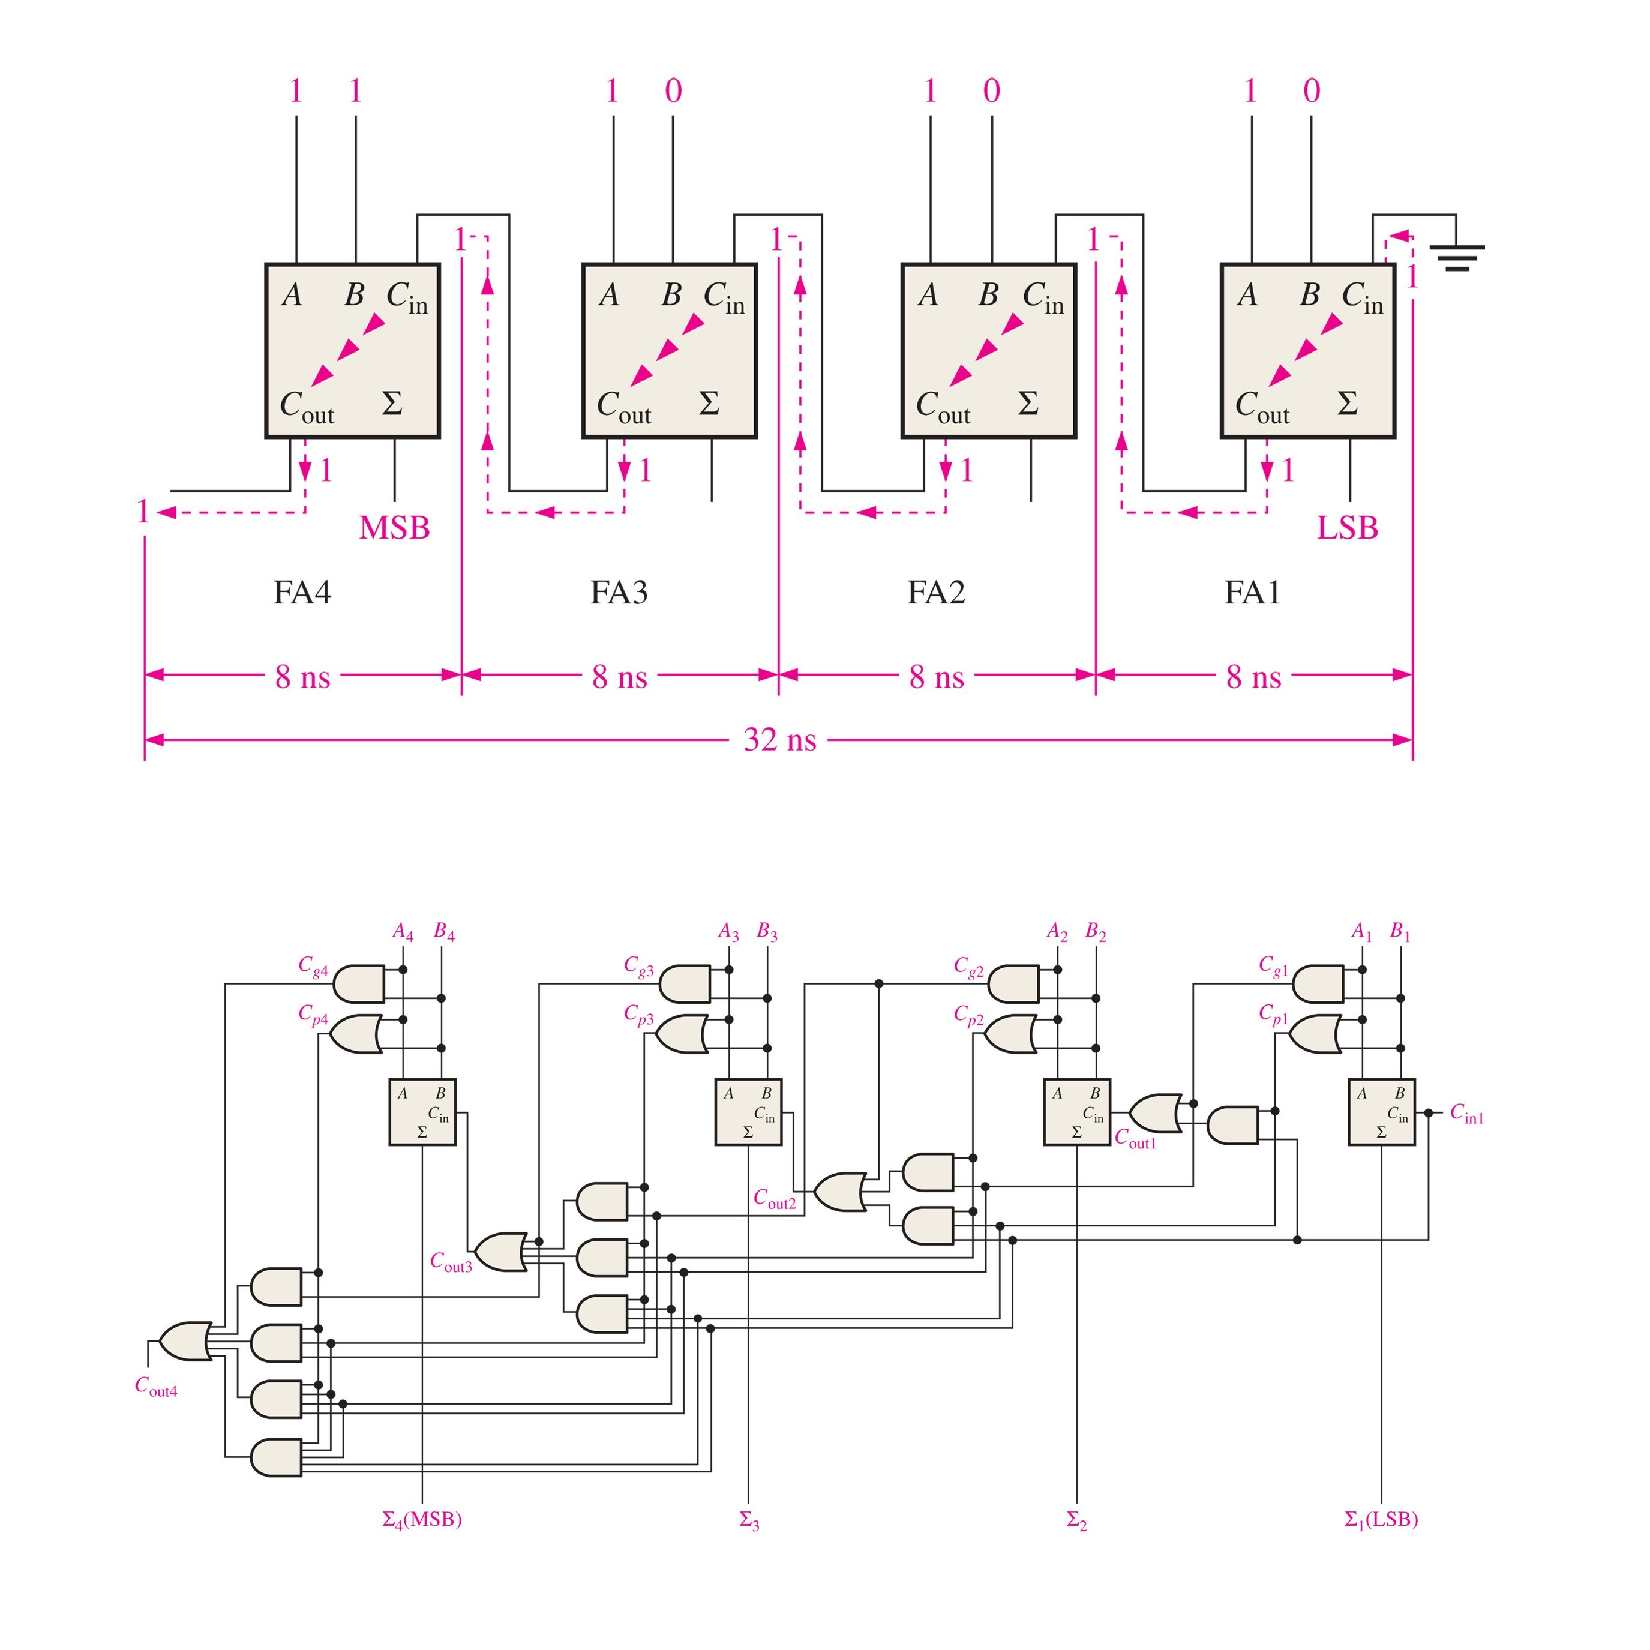
\includegraphics[width=0.5\textwidth]{figures/adder9.pdf}
\caption{\label{fig:add9} Propagation delays add serially in a full-adder with ripple carry topology.}
\end{figure}
\end{frame}

\begin{frame}{Half-Adders and Full-Adders, Ripple-Carry}
\begin{figure}
\centering
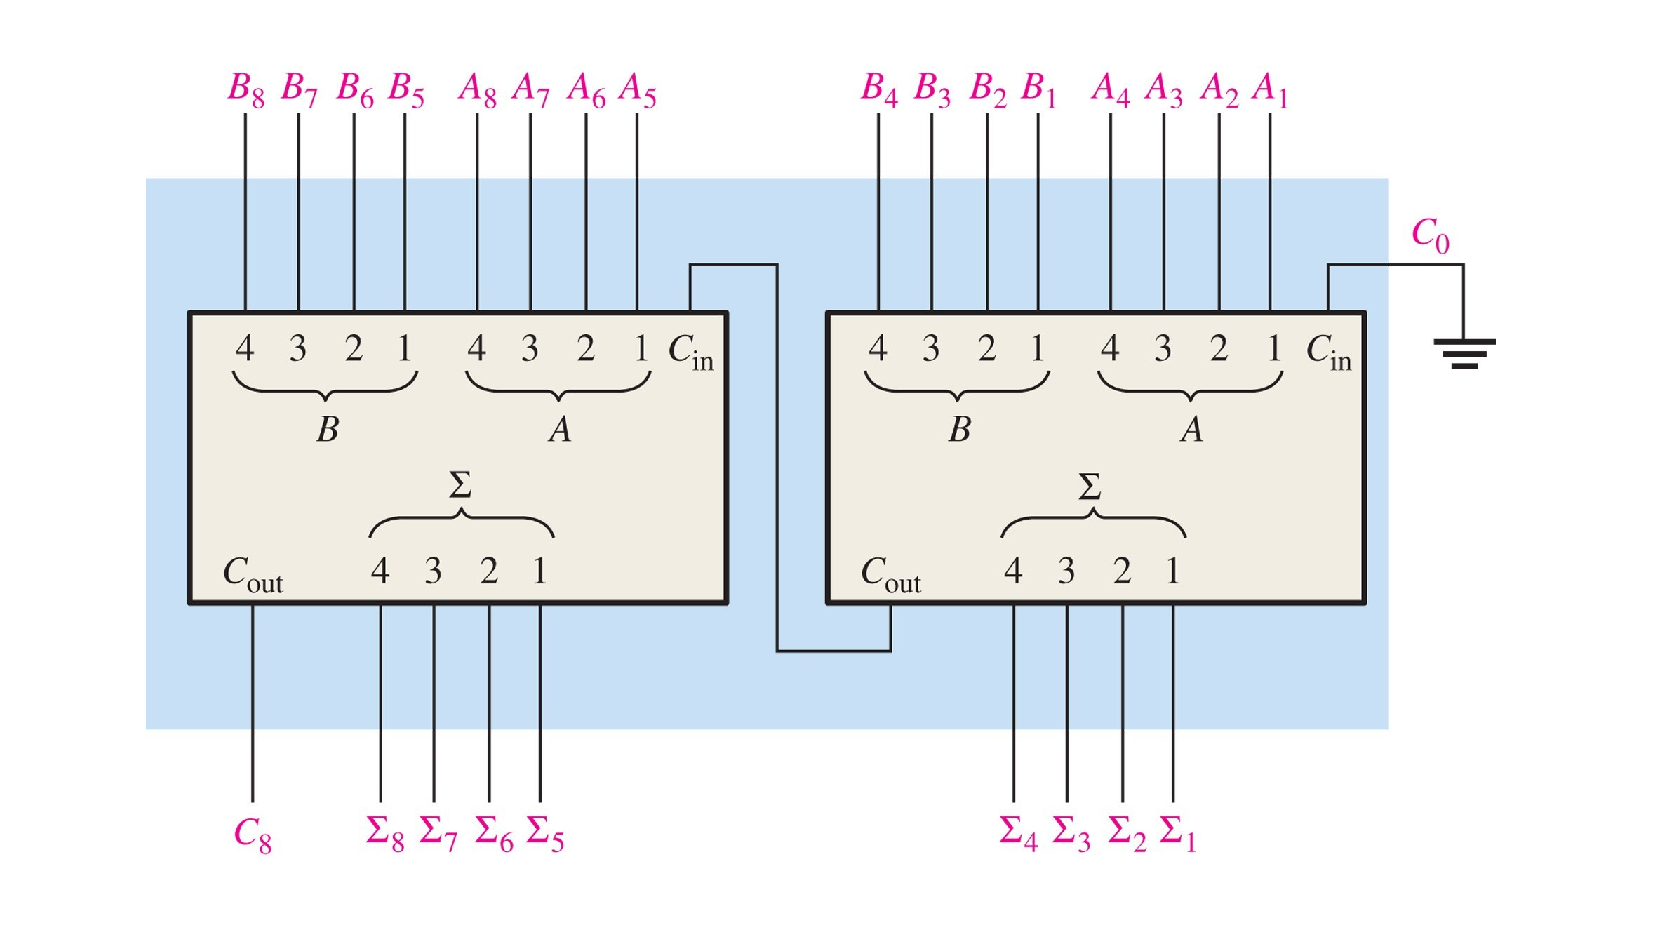
\includegraphics[width=0.75\textwidth]{figures/adder10.pdf}
\caption{\label{fig:add10} Two 4-bit FA connected to form an 8-bit FA, accounting for carries.}
\end{figure}
\end{frame}

\section{Comparators}

\begin{frame}{Comparators}
\begin{figure}
\centering
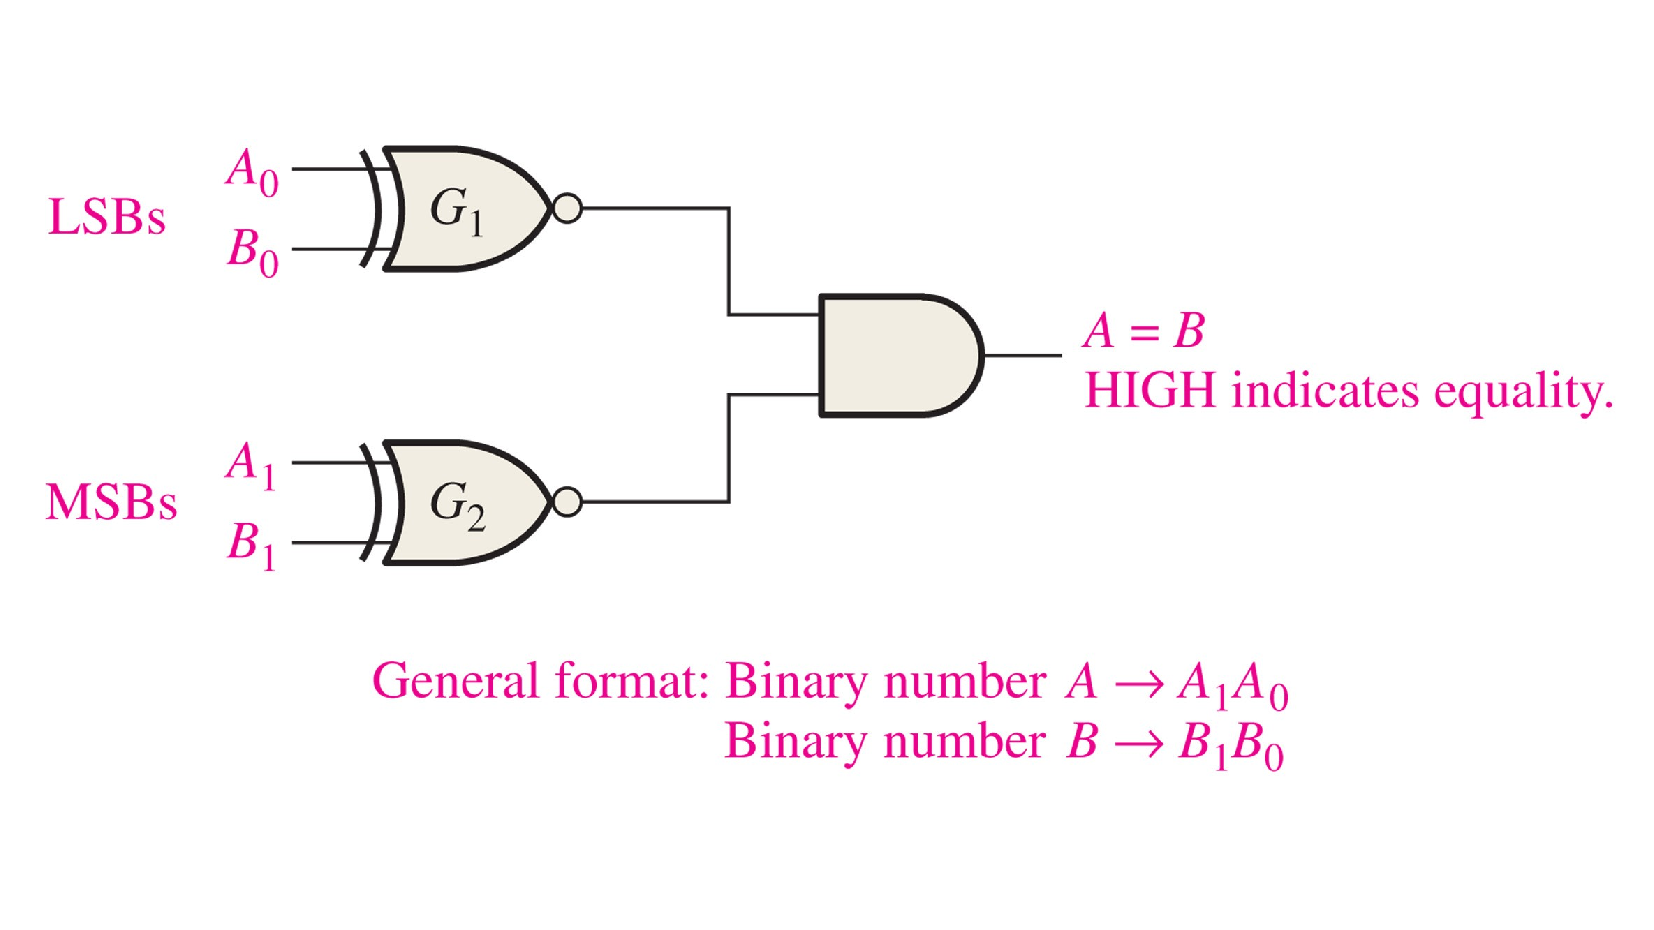
\includegraphics[width=0.75\textwidth]{figures/comparator1.pdf}
\caption{\label{fig:comparator1} The basic idea behind the comparator.  (a) Review the truth table for the XNOR-gate, which is the conjugate of the XOR gate. (b) What is the function of the AND gate?}
\end{figure}
\end{frame}

\begin{frame}{Comparators}
\begin{figure}
\centering
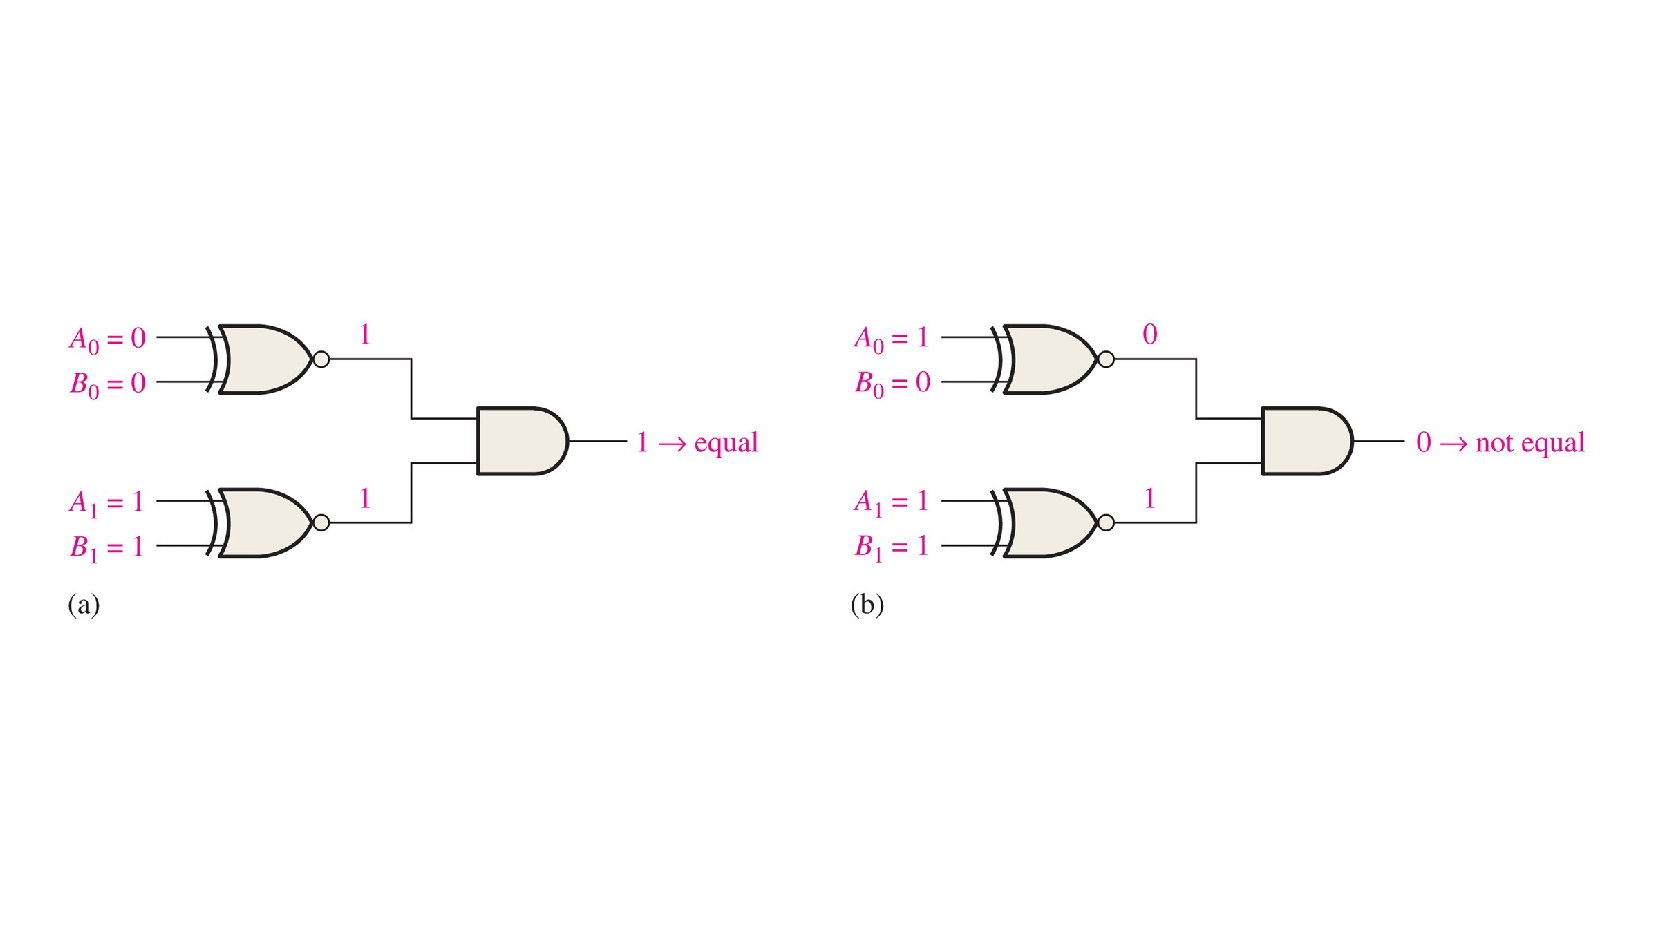
\includegraphics[width=0.9\textwidth,trim=0cm 3cm 0cm 3cm,clip=true]{figures/comparator2.pdf}
\caption{\label{fig:comparator2} (a) Example of comparison of 2-bit binary numbers.  (b) What is the truth table? (c) What is the logical representation of the function?  (c) What is a logical representation for the inequality circuit?}
\end{figure}
\end{frame}

\begin{frame}{Comparators}
\begin{figure}
\centering
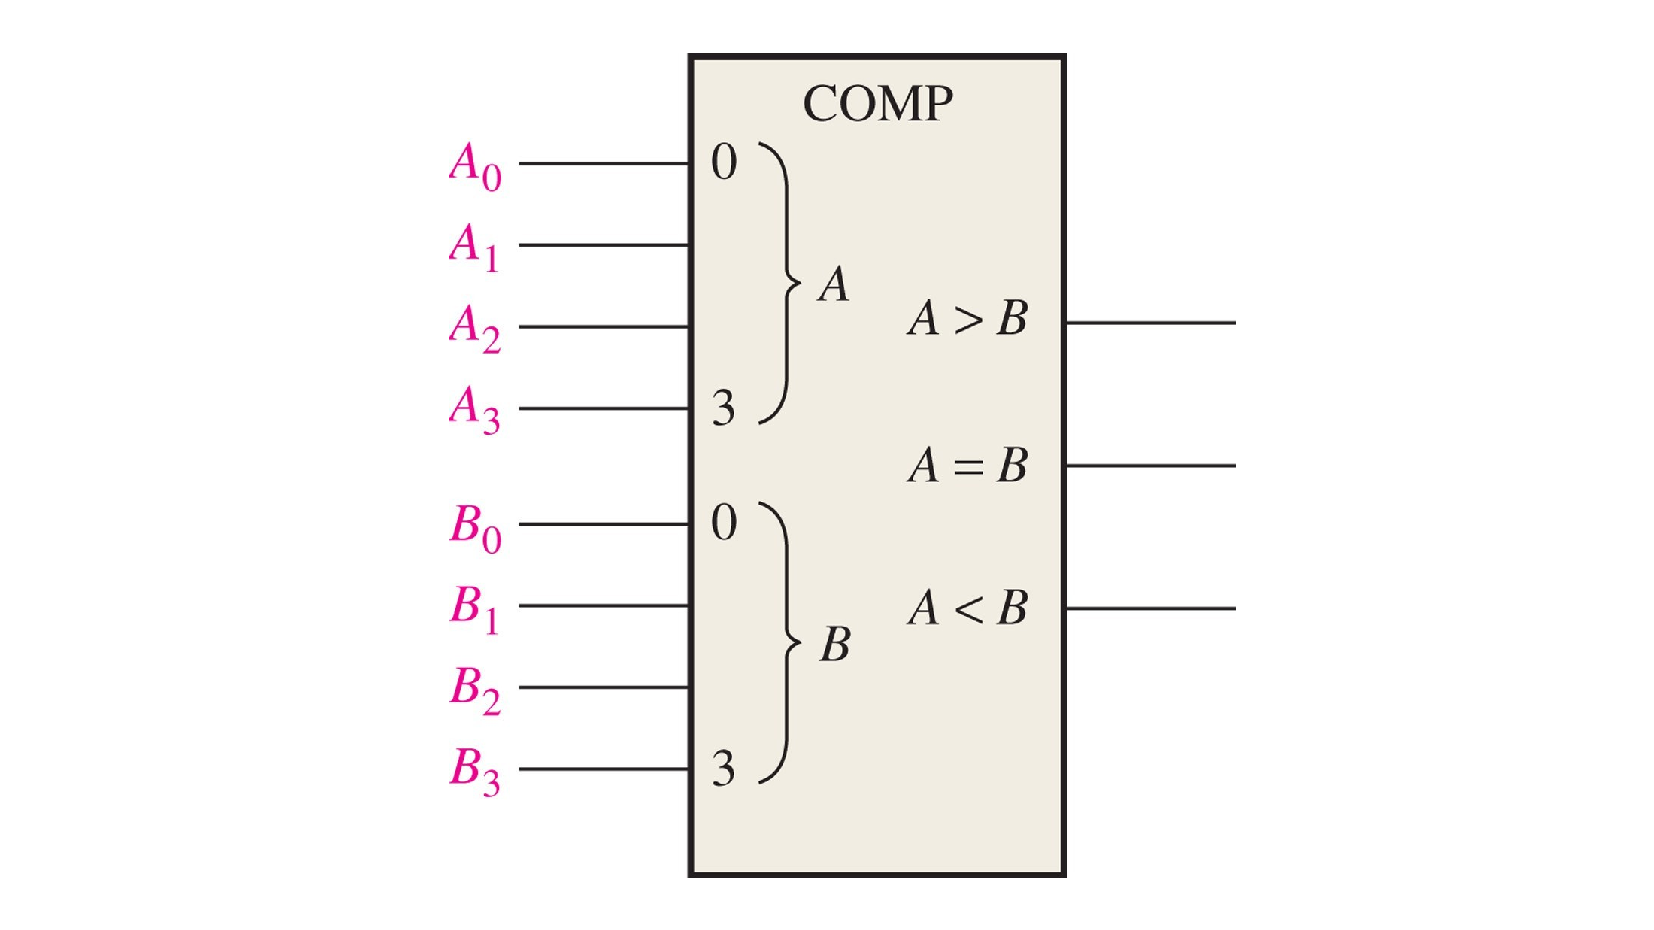
\includegraphics[width=0.45\textwidth,trim=3cm 0cm 3cm 0cm,clip=true]{figures/comparator3.pdf} \hspace{0.25cm}
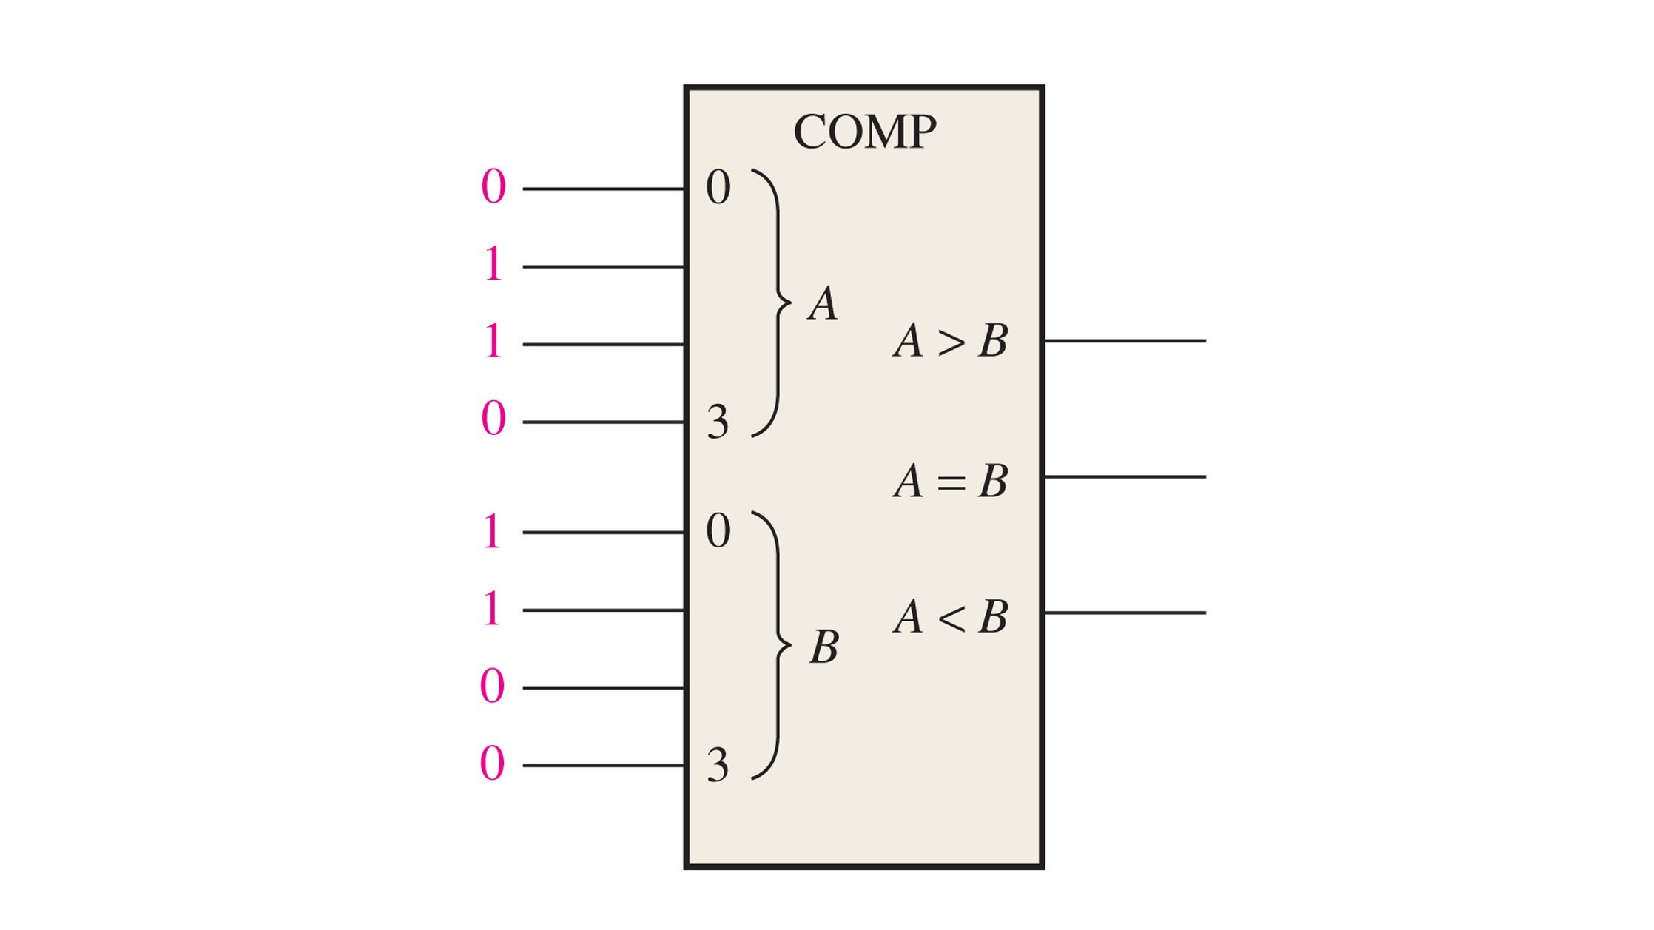
\includegraphics[width=0.45\textwidth,trim=3cm 0cm 3cm 0cm,clip=true]{figures/comparator4.pdf}
\caption{\label{fig:comparator3} (Left) One \textit{component} that is really 8 comparators linked to the same AND gate. (Right) What is the correct ouput? How to determine the inequality functions?}
\end{figure}
\end{frame}

\begin{frame}{Comparators}
\begin{figure}
\centering
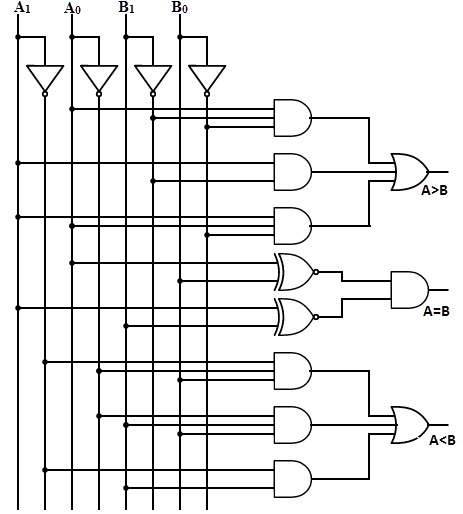
\includegraphics[width=0.5\textwidth]{figures/2bitcomp.jpg}
\caption{\label{fig:comparator4} Try some simple cases: (a) A = 00 and B = 01, (b) A = 10 and B = 01.}
\end{figure}
\end{frame}

\section{Decoders}

\begin{frame}{Decoders}
\begin{figure}
\centering
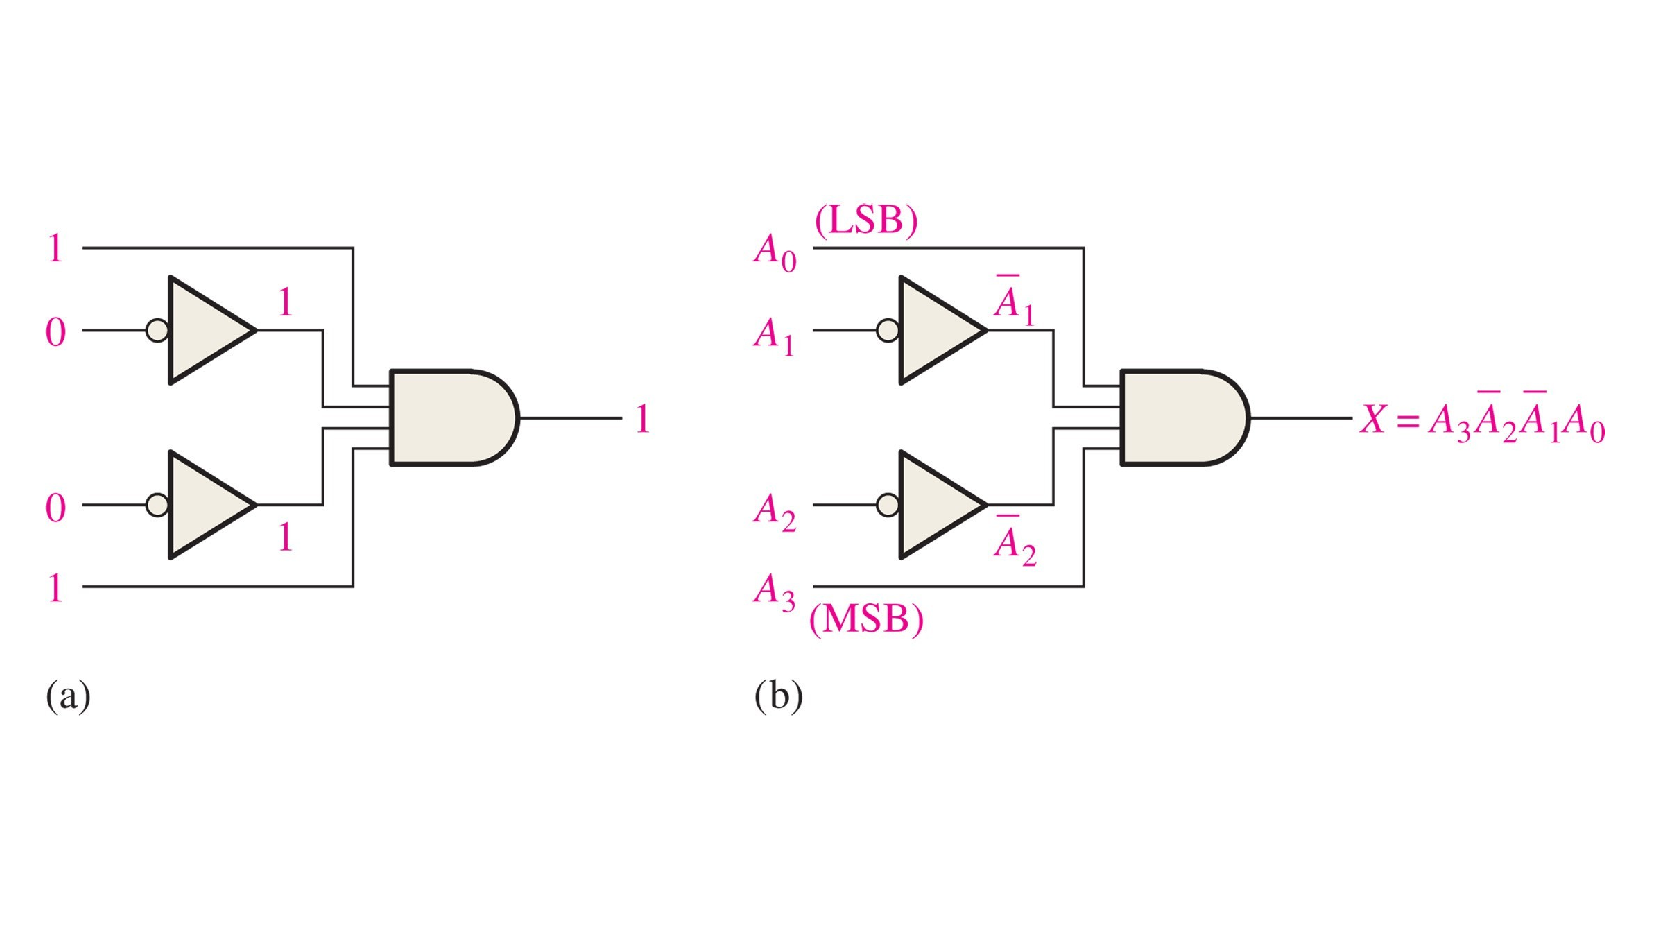
\includegraphics[width=0.75\textwidth]{figures/decoder1.pdf}
\caption{\label{fig:decoder1} The binary decoder circuit for 9.  This circuit is true if the binary number is 1001.  (Pay attention to the order of MSB and LSB).}
\end{figure}
\end{frame}

\begin{frame}{Decoders}
\begin{figure}
\centering
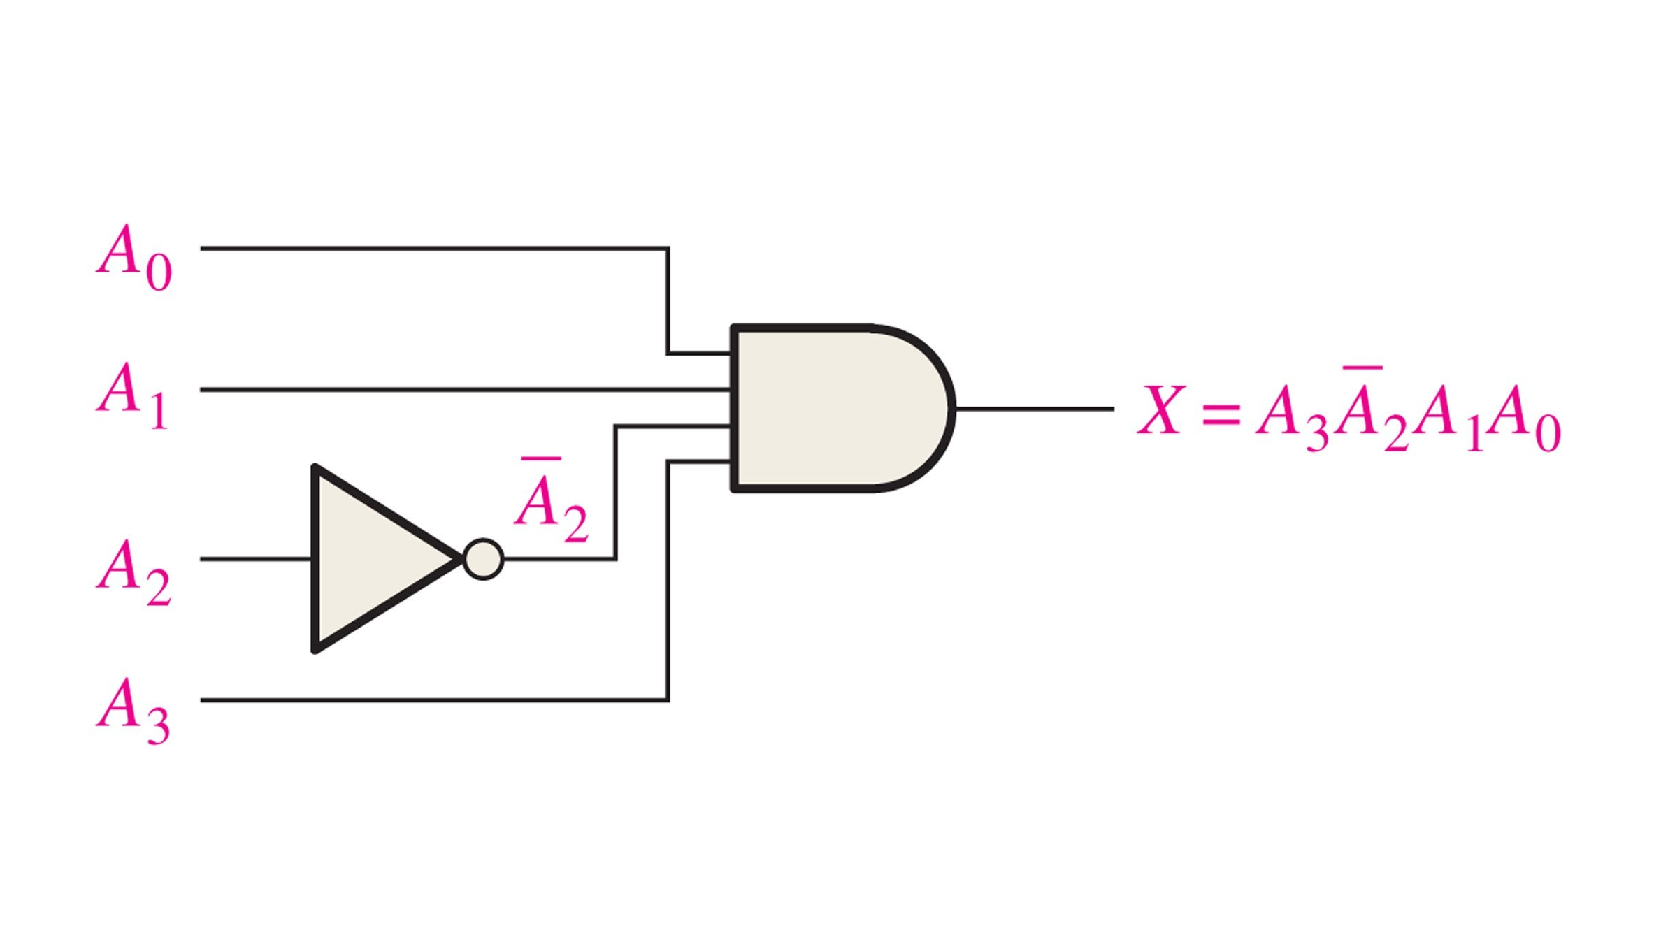
\includegraphics[width=0.75\textwidth]{figures/decoder2.pdf}
\caption{\label{fig:decoder2} (a) Which binary number is being decoded here? (b) What would it take to decode all binary numbers of $n$ bits?}
\end{figure}
\end{frame}

\begin{frame}{Decoders}
\begin{figure}
\centering
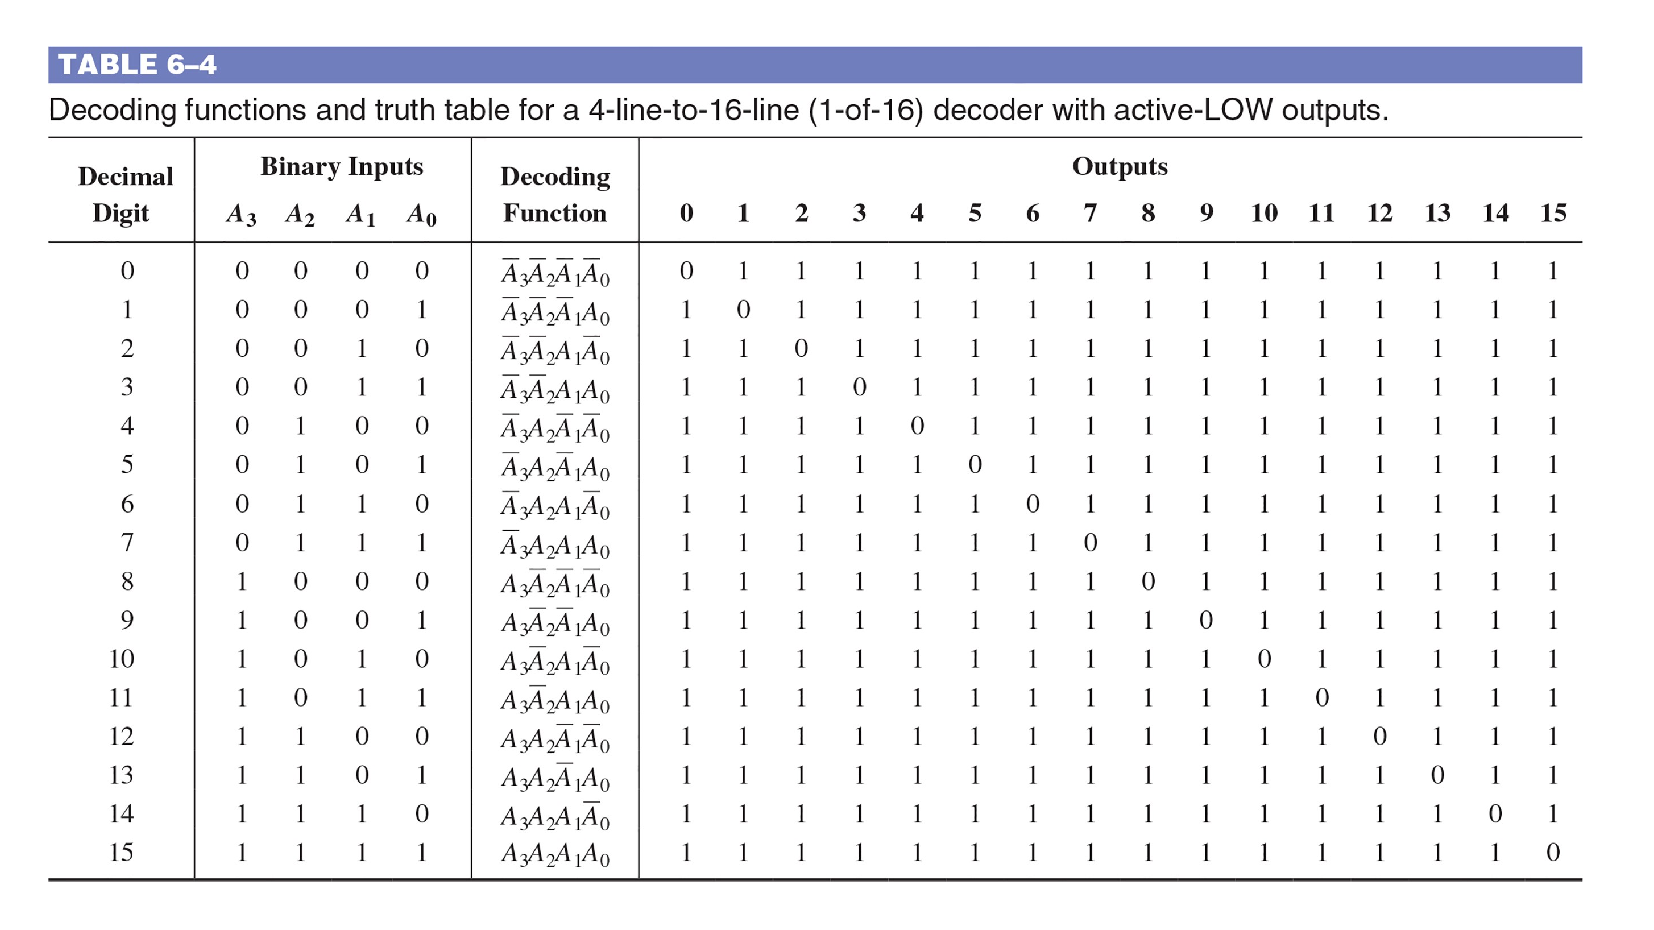
\includegraphics[width=0.85\textwidth]{figures/decoder3.pdf}
\caption{\label{fig:decoder3} The decoding table for ACTIVE LOW 4-bit binary.  Terms from linear algebra: this matrix has 0 trace, and is symmetric (we can exchange rows and columns).}
\end{figure}
\end{frame}

\section{Encoders}

\begin{frame}{Encoders}
\begin{figure}
\centering
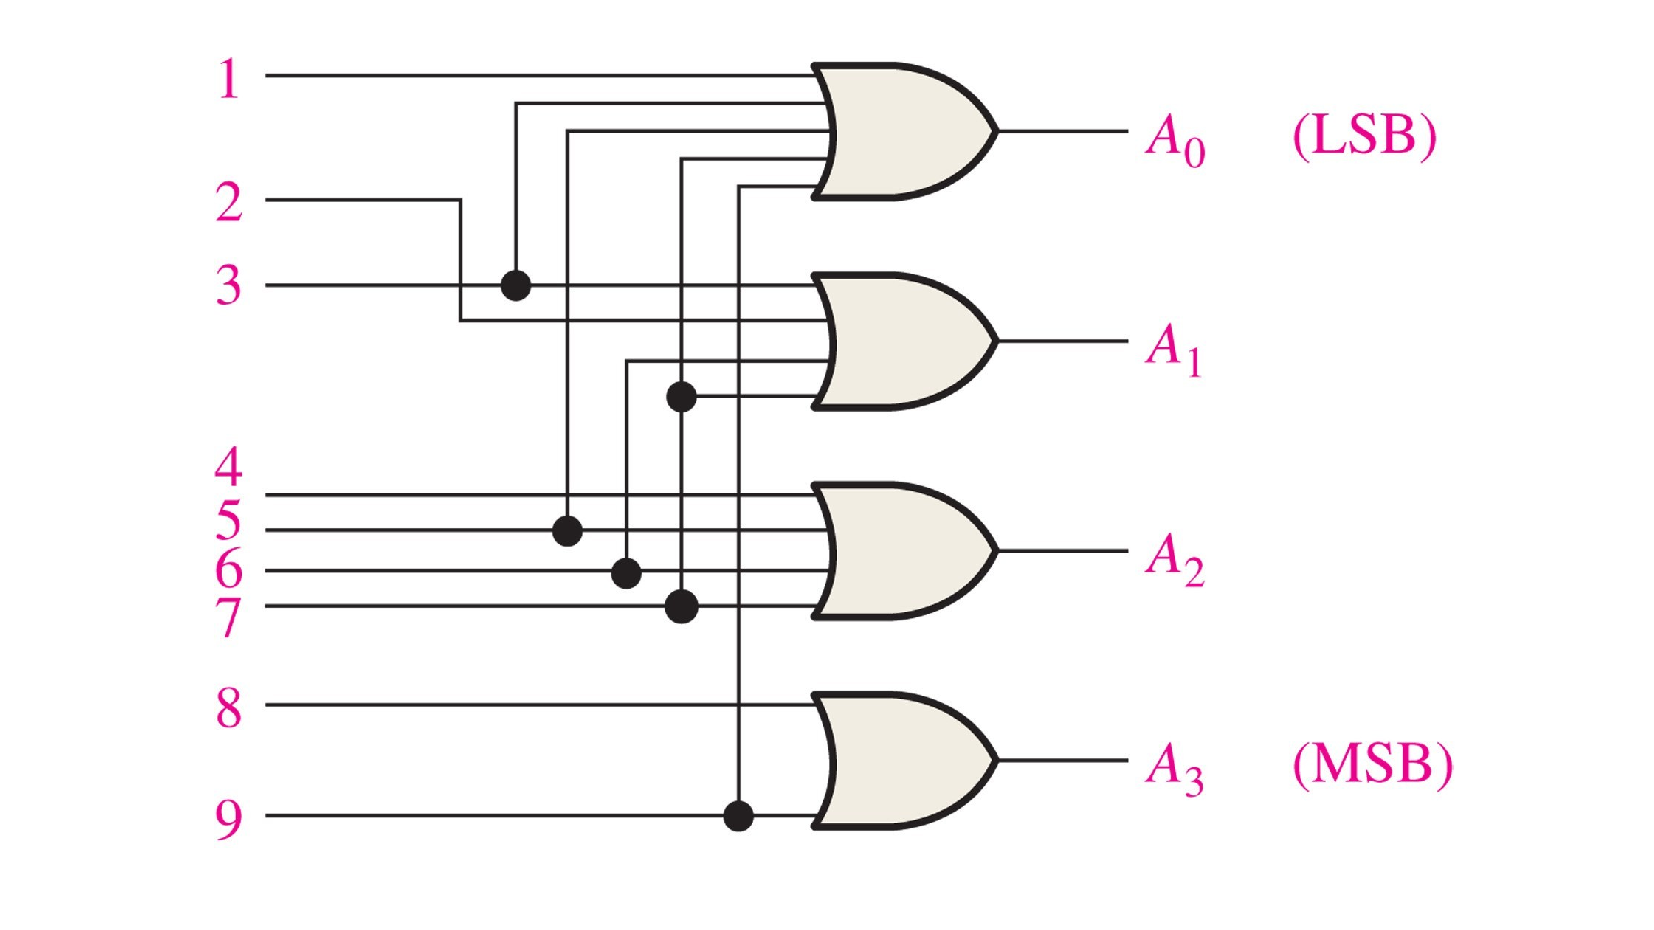
\includegraphics[width=0.85\textwidth]{figures/encoder1.pdf}
\caption{\label{fig:encoder1} Recall the OR TT, and remember that this is a system in which there are forbidden or \textit{don't care} states.  Only one input line can be active at once.}
\end{figure}
\end{frame}

\begin{frame}{Encoders}
\begin{figure}
\centering
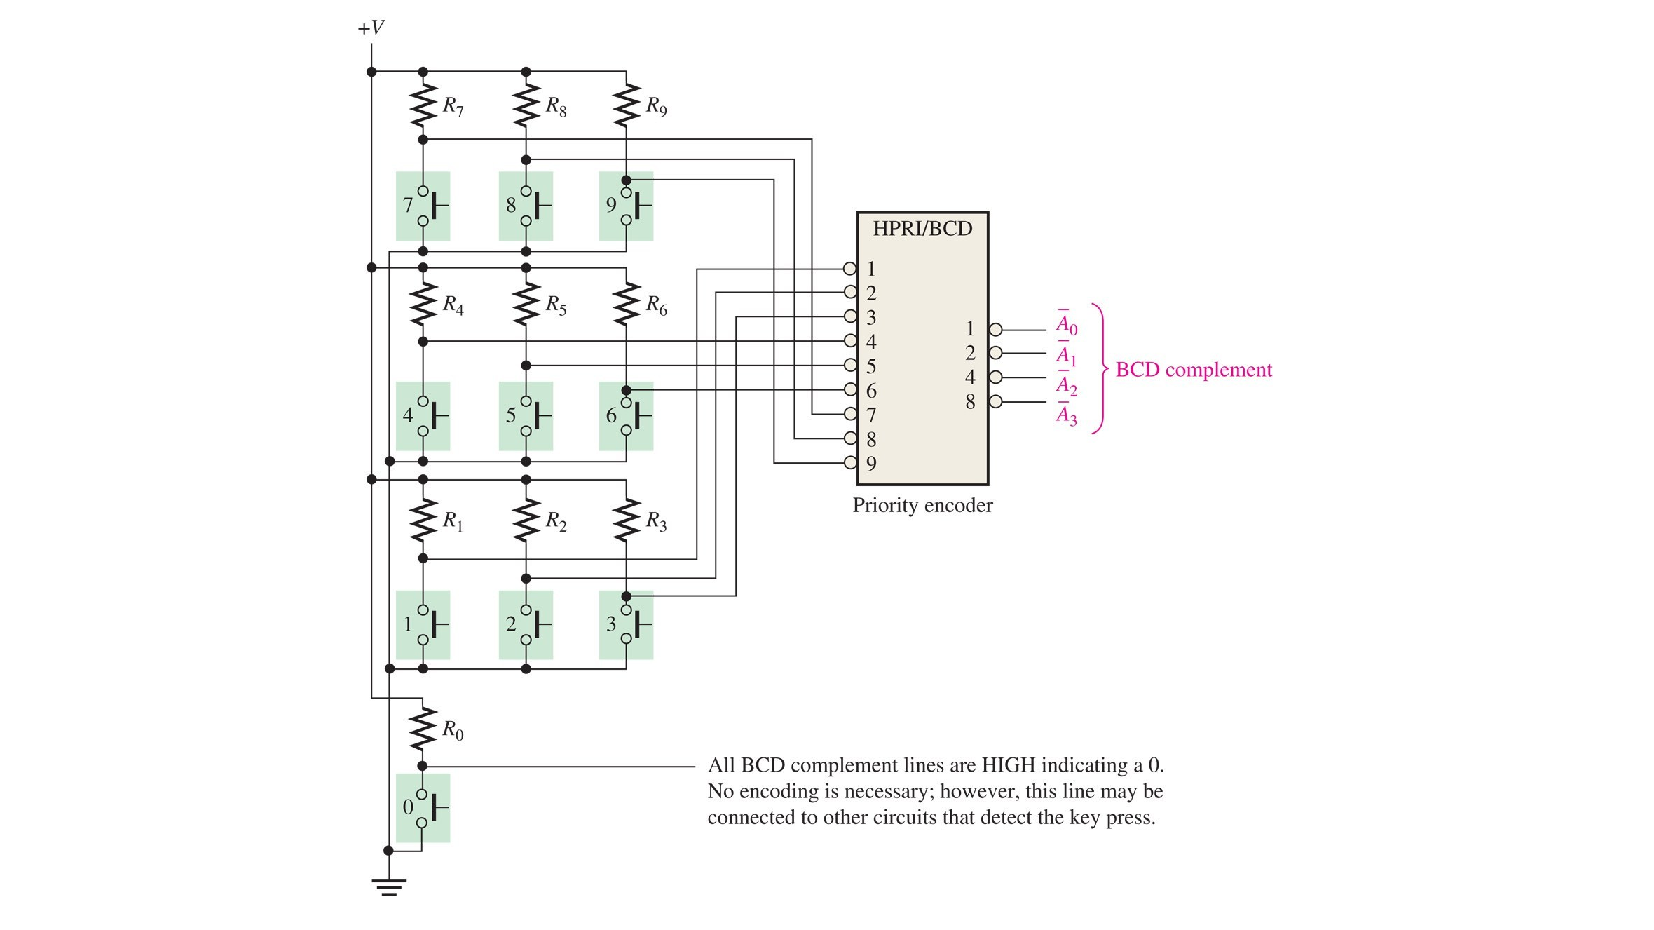
\includegraphics[width=0.75\textwidth,trim=3cm 0cm 3cm 0cm,clip=true]{figures/encoder2.pdf}
\caption{\label{fig:encoder2} A keypad system.  The binary encoder accepts only 9 digits because 0 is redundant.  Note the use of \textit{pull-up} resistors (recall LEDs operations).}
\end{figure}
\end{frame}

\section{Multiplexers}

\begin{frame}{Multiplexers}
\begin{figure}
\centering
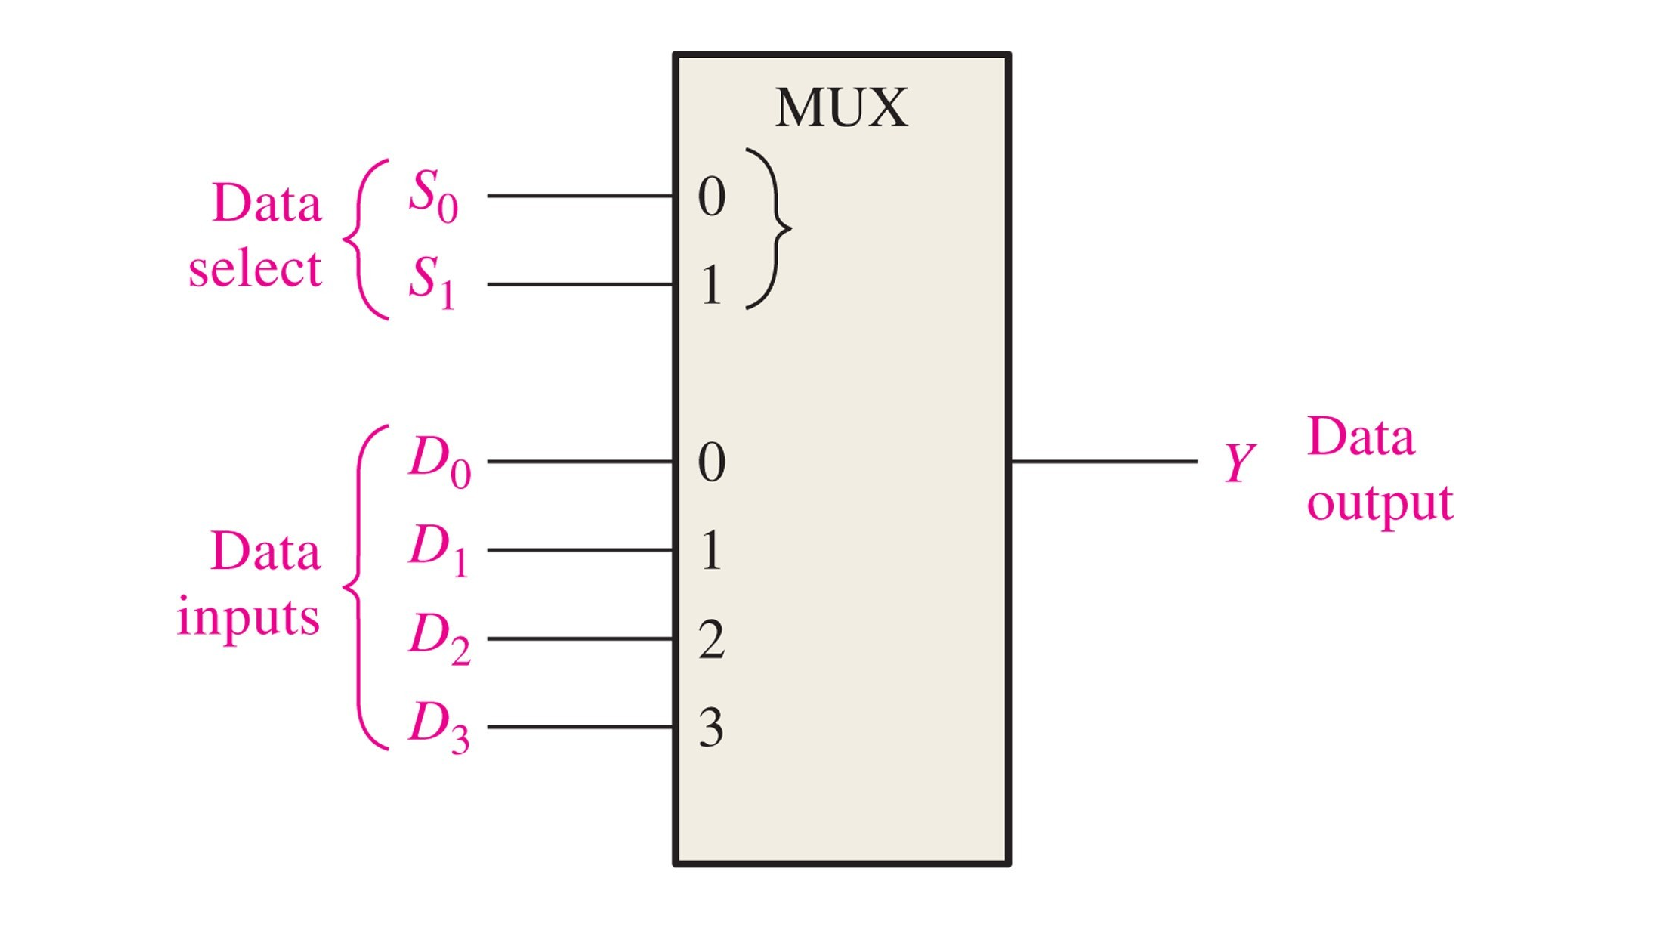
\includegraphics[width=0.75\textwidth,trim=3cm 0cm 3cm 0cm,clip=true]{figures/mux1.pdf}
\caption{\label{fig:mux1} A general block diagram for a \textit{multiplexer.}  Parallel data input is successively rotated to the single output.}
\end{figure}
\end{frame}

\begin{frame}{Multiplexers}
\begin{figure}
\centering
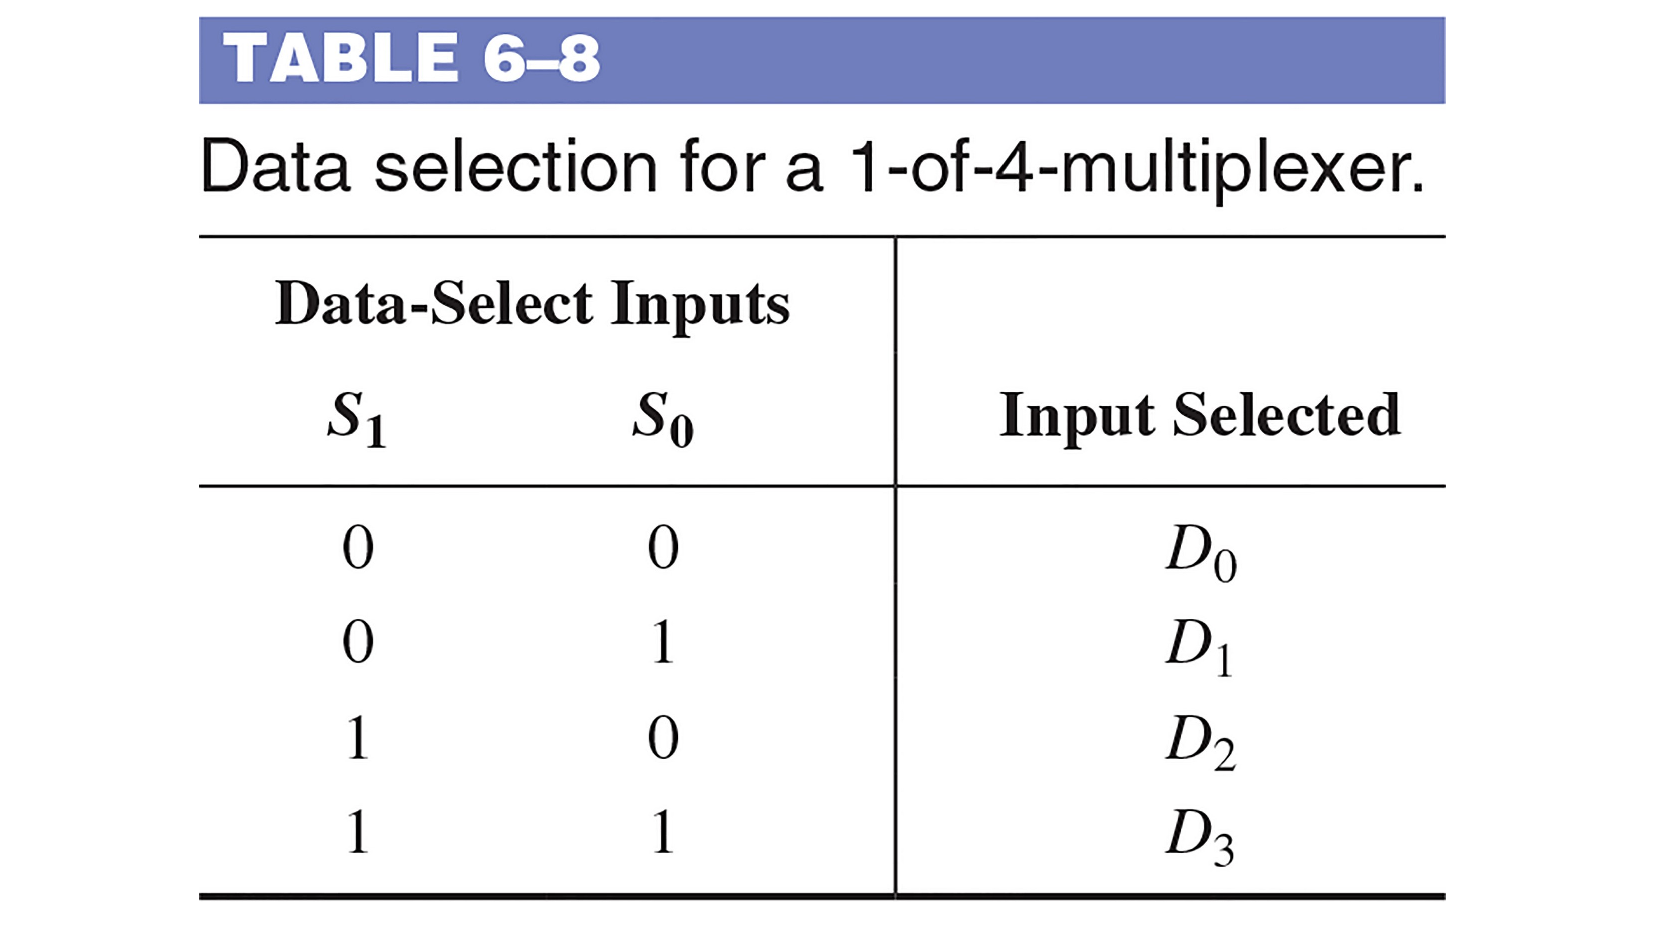
\includegraphics[width=0.75\textwidth,trim=3cm 0cm 3cm 0cm,clip=true]{figures/mux2.pdf}
\caption{\label{fig:mux2} The desired TT for a 1-of-4 mux.  The n-of-m jargon corresponds to inputs and outputs.  We should also have \textit{enable}, and one or more output lines.}
\end{figure}
\end{frame}

\begin{frame}{Multiplexers}
\begin{figure}
\centering
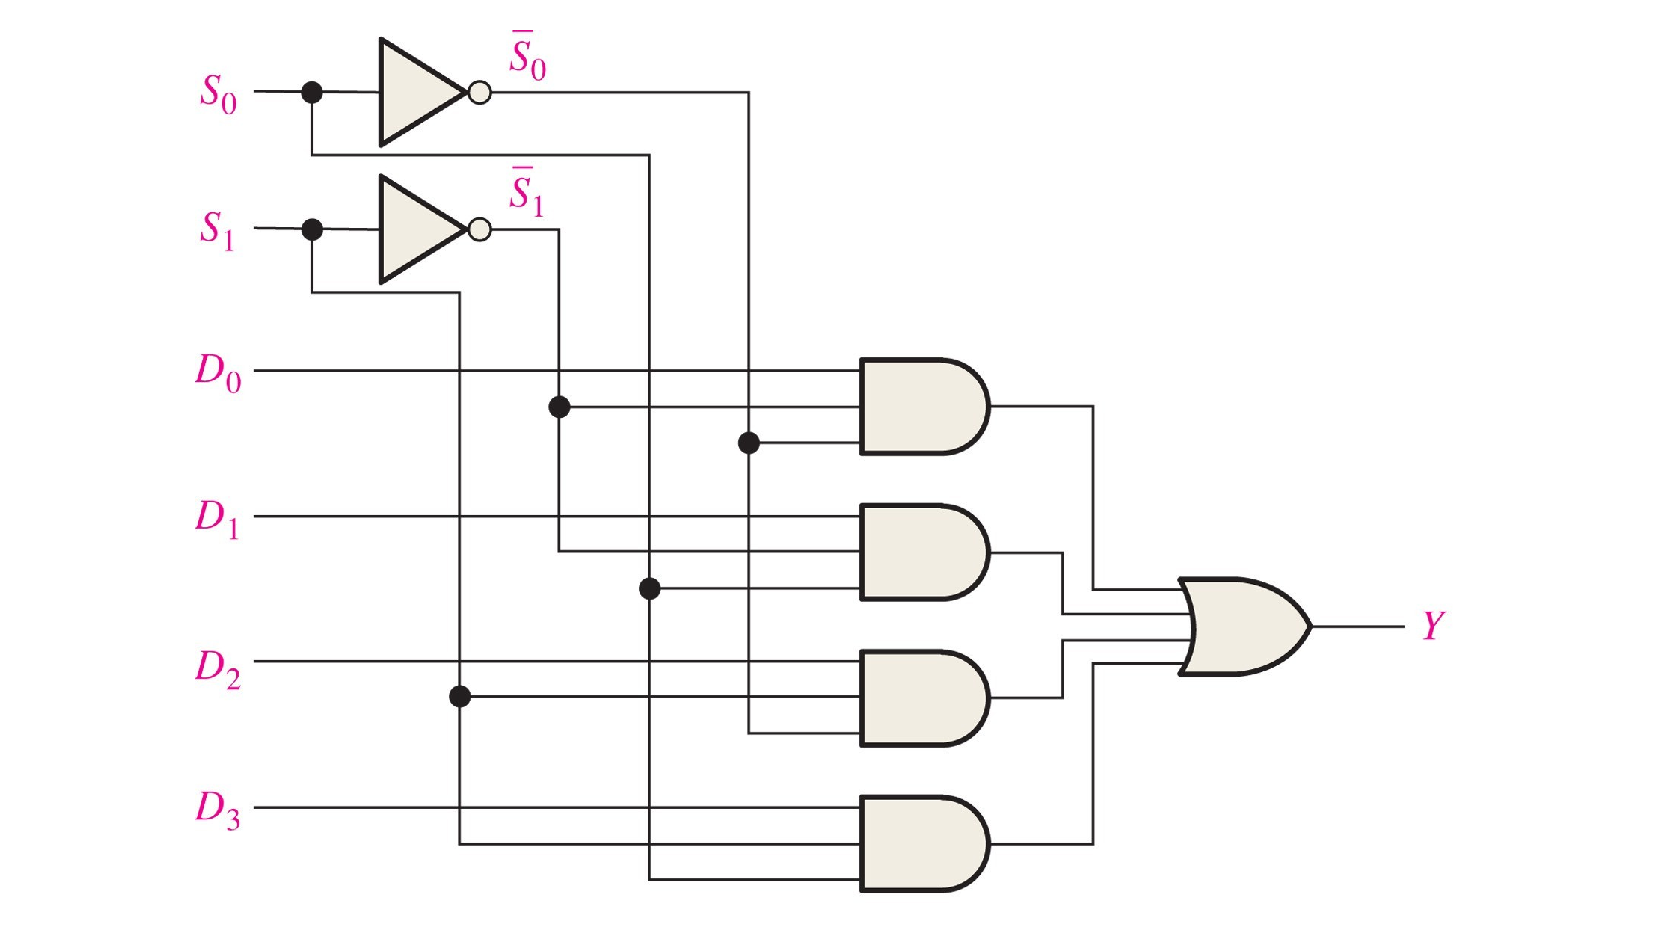
\includegraphics[width=0.75\textwidth,trim=3cm 0cm 3cm 0cm,clip=true]{figures/mux3.pdf}
\caption{\label{fig:mux3} The AND-enable behavior is used in this 1-of-4 mux.  Note the interconnections are the key to generating the right output logic.}
\end{figure}
\end{frame}

\begin{frame}{Multiplexers}
\begin{figure}
\centering
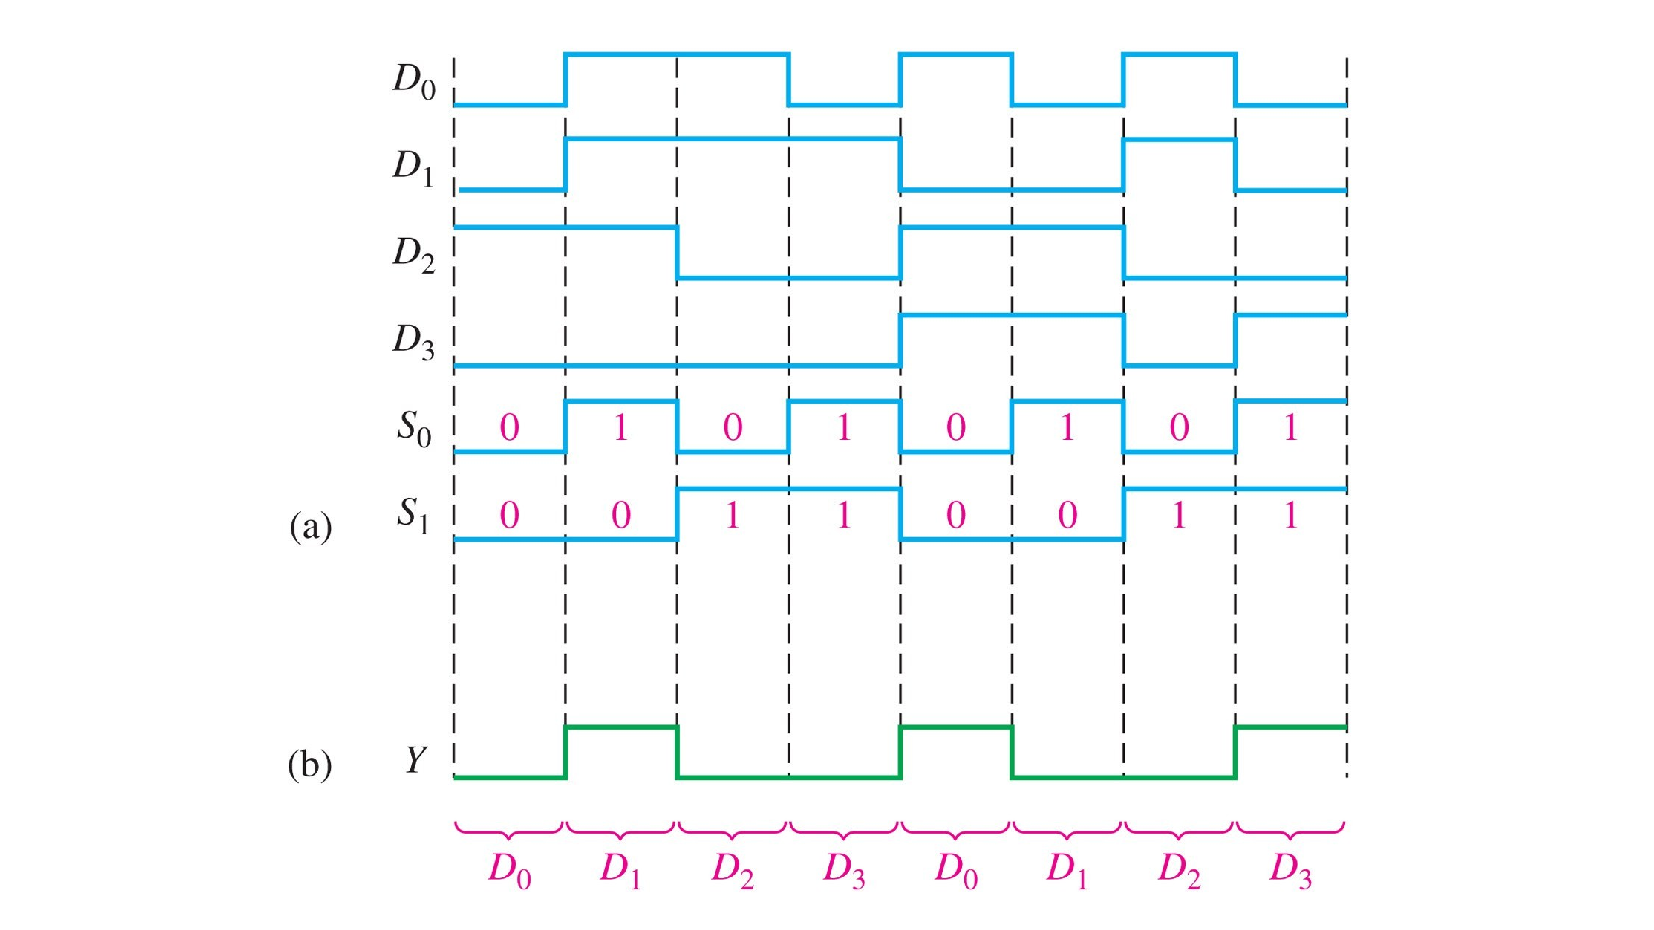
\includegraphics[width=0.75\textwidth,trim=3cm 0cm 3cm 0cm,clip=true]{figures/mux4.pdf}
\caption{\label{fig:mux4} Exercise: verify the timing diagram output Y follows the 1-of-4 pattern.  The data-select lines follow a 2-bit \textit{counter} (coming soon).}
\end{figure}
\end{frame}

\begin{frame}{Multiplexers}
\begin{figure}
\centering
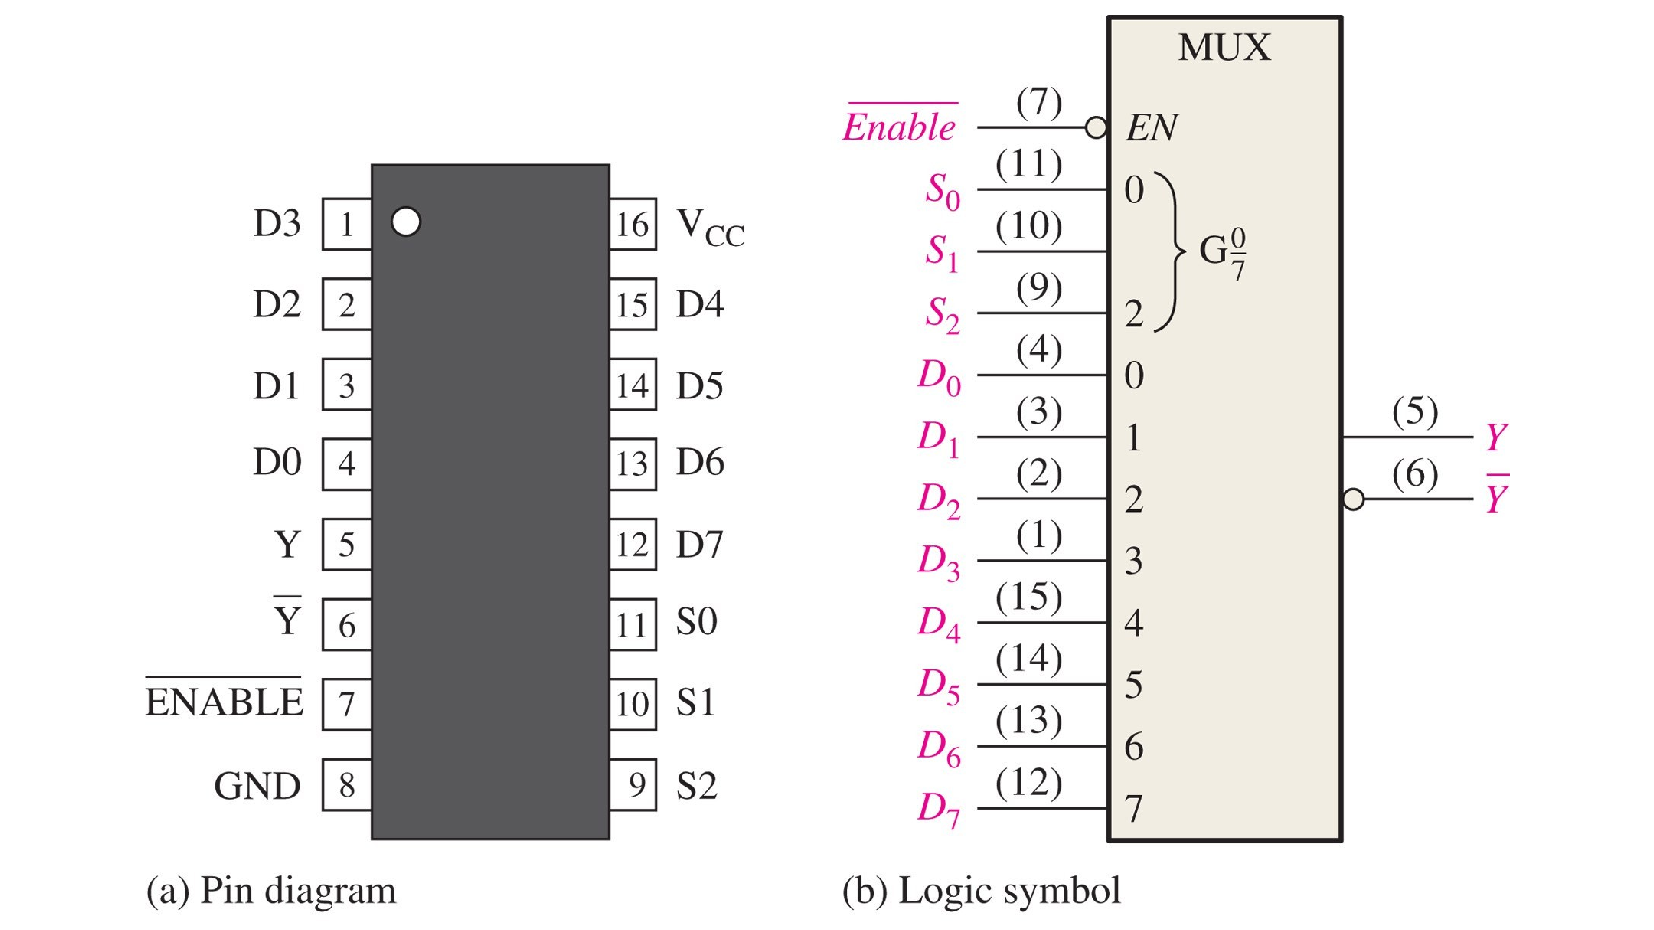
\includegraphics[width=0.75\textwidth,trim=3cm 0cm 3cm 0cm,clip=true]{figures/mux5.pdf}
\caption{\label{fig:mux5} Active LOW enabled, 1-of-8 mux with complemented output.}
\end{figure}
\end{frame}

\begin{frame}{Multiplexers}
\begin{figure}
\centering
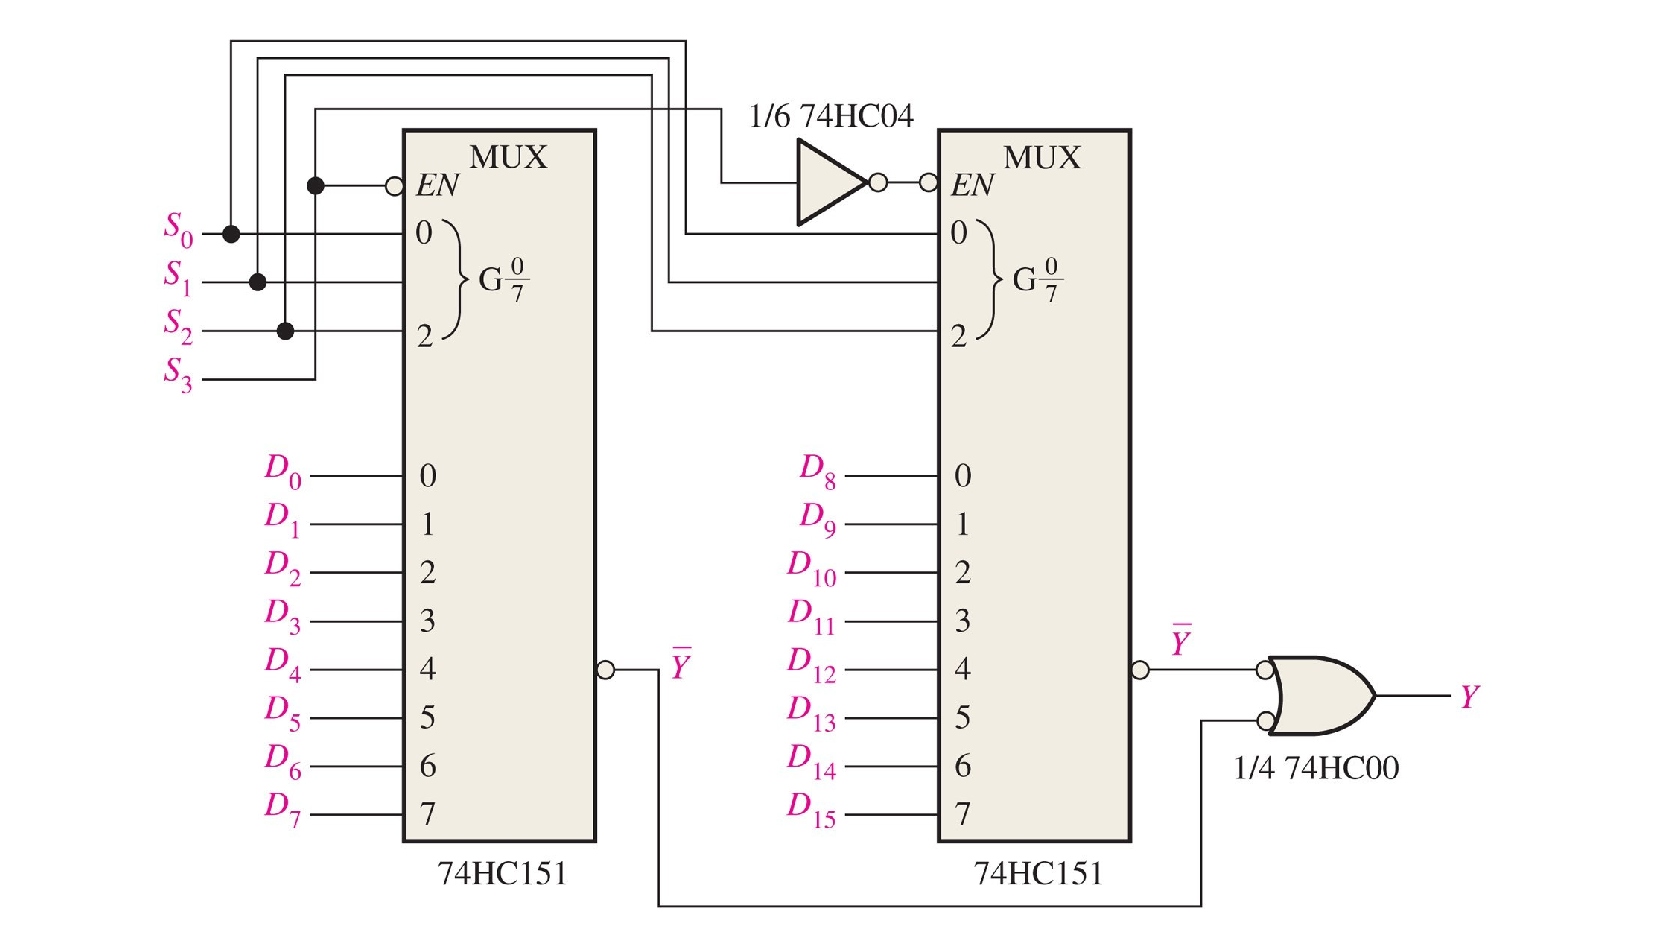
\includegraphics[width=0.75\textwidth,trim=3cm 0cm 3cm 0cm,clip=true]{figures/mux6.pdf}
\caption{\label{fig:mux6} Active LOW enabled, 1-of-8 mux with complemented output, connected to another one.  The overall system acts as a 1-of-16 with 4 data select lines.}
\end{figure}
\end{frame}

\begin{frame}{Multiplexers}
\begin{figure}
\centering
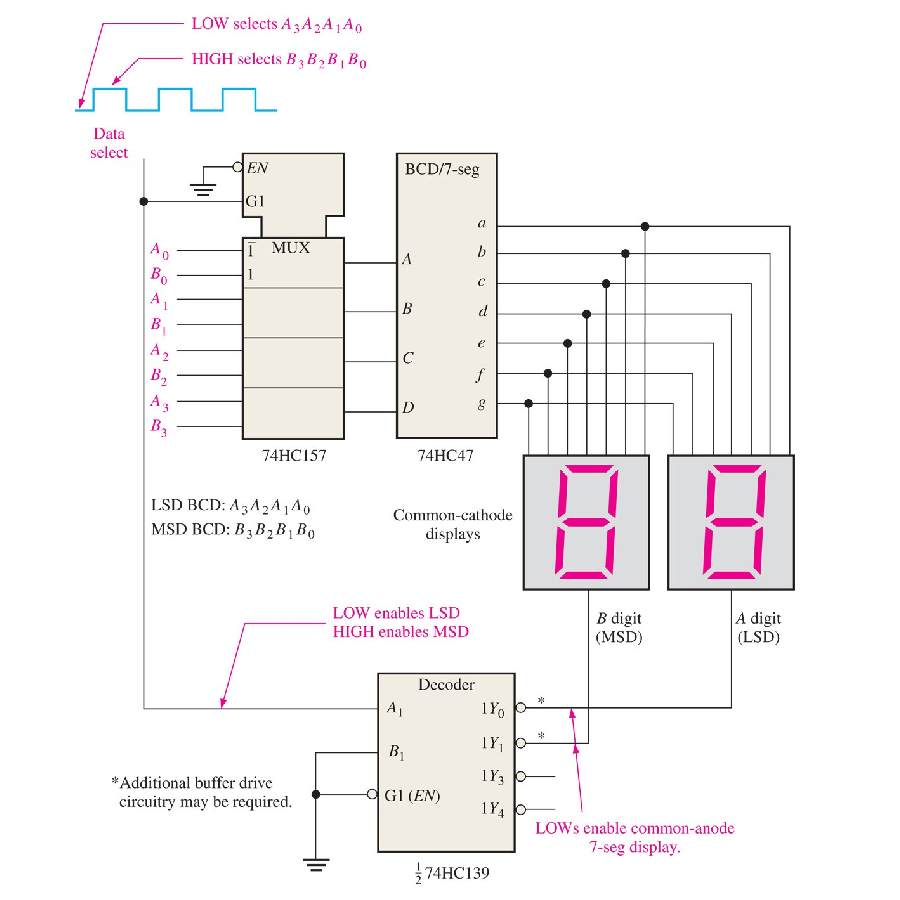
\includegraphics[width=0.55\textwidth]{figures/mux7.pdf}
\caption{\label{fig:mux7} In this example, the mux is a \textit{quad} 1-of-2, to help switch between binary numbers A and B.  The BCD decoder converts the inputs, and the 2-to-4 decoder grounds either display.}
\end{figure}
\end{frame}

\begin{frame}{Multiplexers}
\begin{figure}
\centering
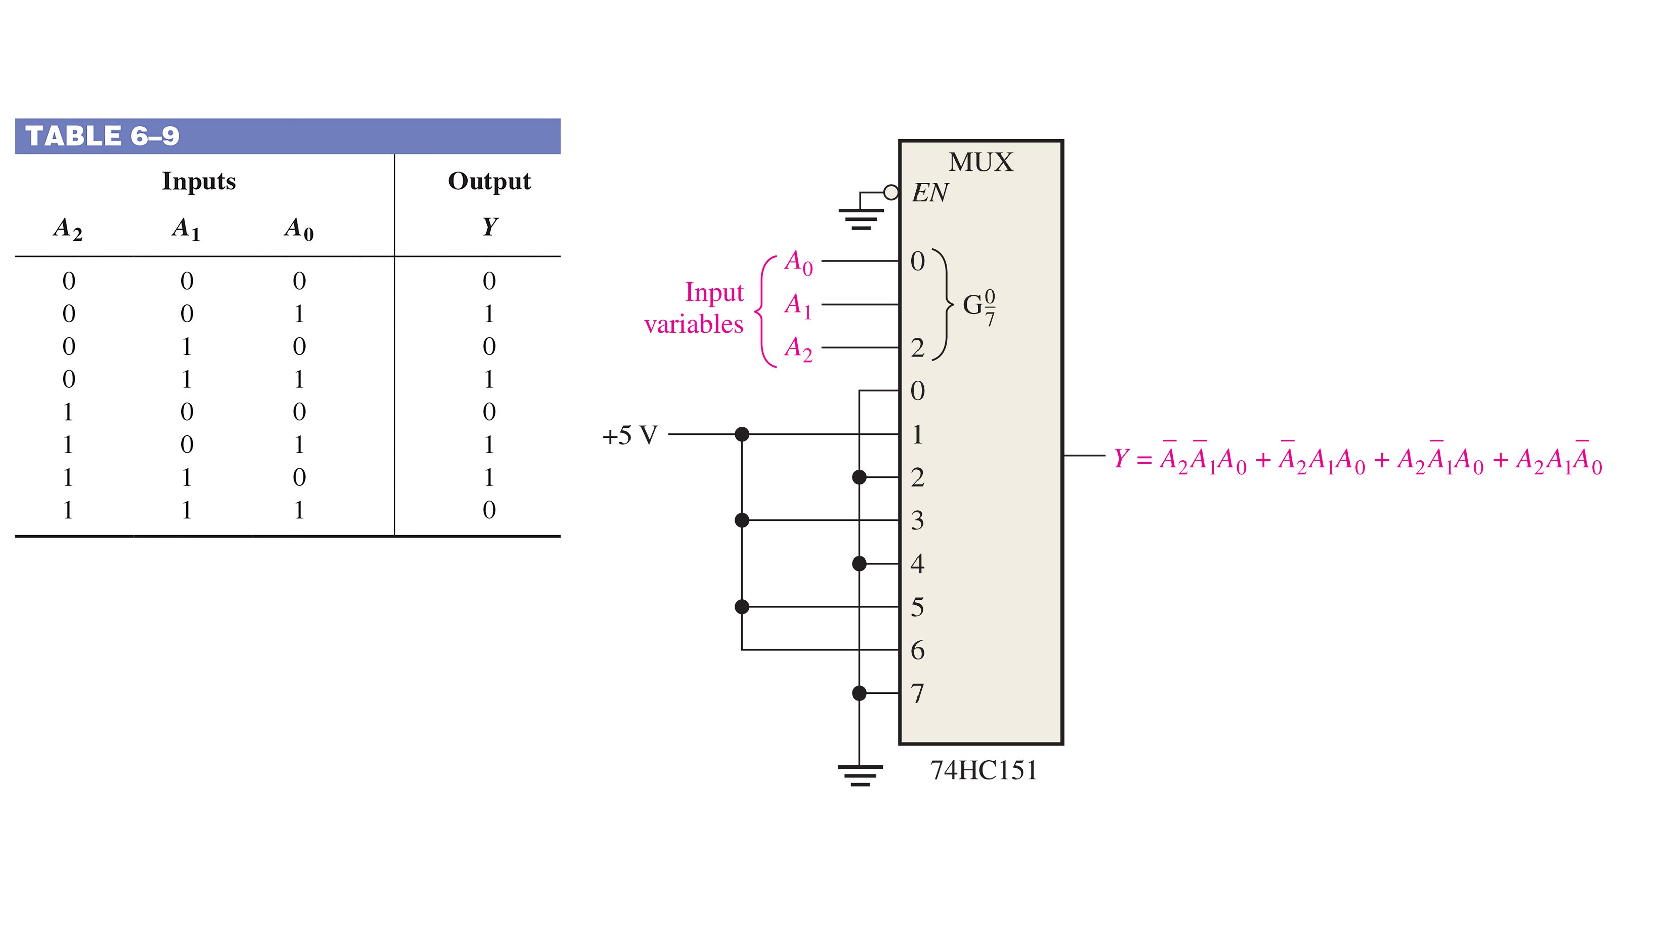
\includegraphics[width=0.95\textwidth,trim=2cm 2cm 0cm 2cm,clip=true]{figures/mux8.pdf}
\caption{\label{fig:mux8} A mux can also be used to create any domain-N logic-function, provided we can connect HIGH and LOW to the desired input lines.  Do you see the pattern?}
\end{figure}
\end{frame}

\section{Demultiplexers}

\begin{frame}{Demultiplexers}
\begin{figure}
\centering
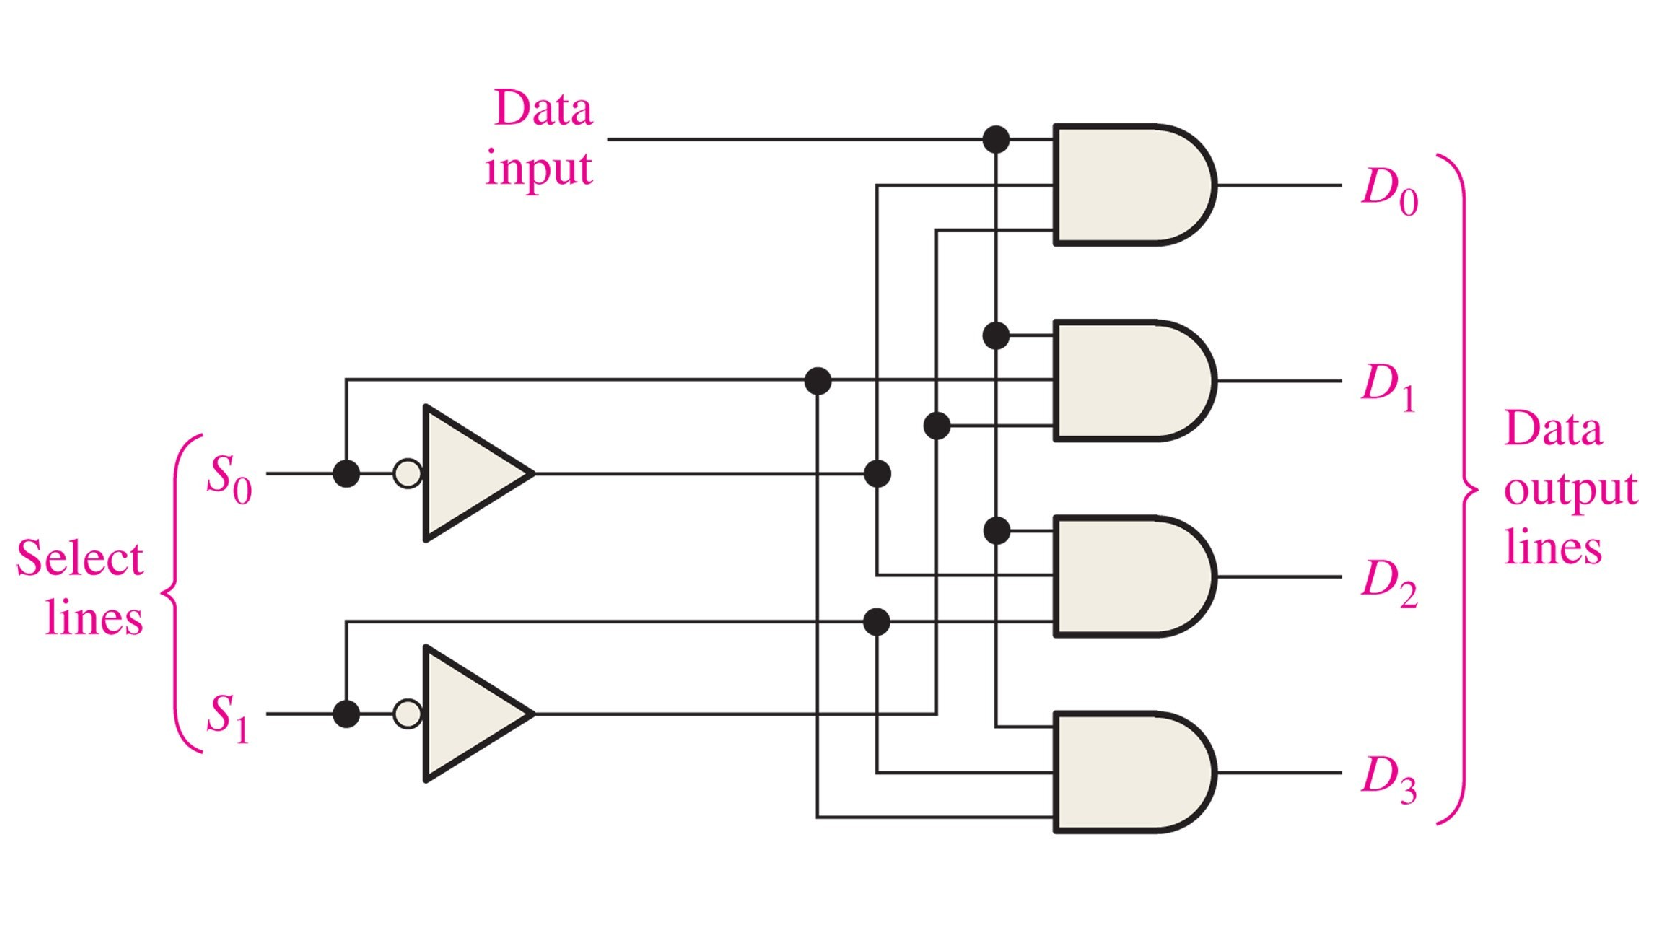
\includegraphics[width=0.75\textwidth,trim=3cm 0cm 3cm 0cm,clip=true]{figures/dmux1.pdf}
\caption{\label{fig:dmux1} The reverse operation to a multiplexer is a demultiplexer, or demux.  Note the AND-enable is still there on the input line, but we need 4 ANDs: 1 for each possible input data line on the mux.}
\end{figure}
\end{frame}

\begin{frame}{Demultiplexers}
\begin{figure}
\centering
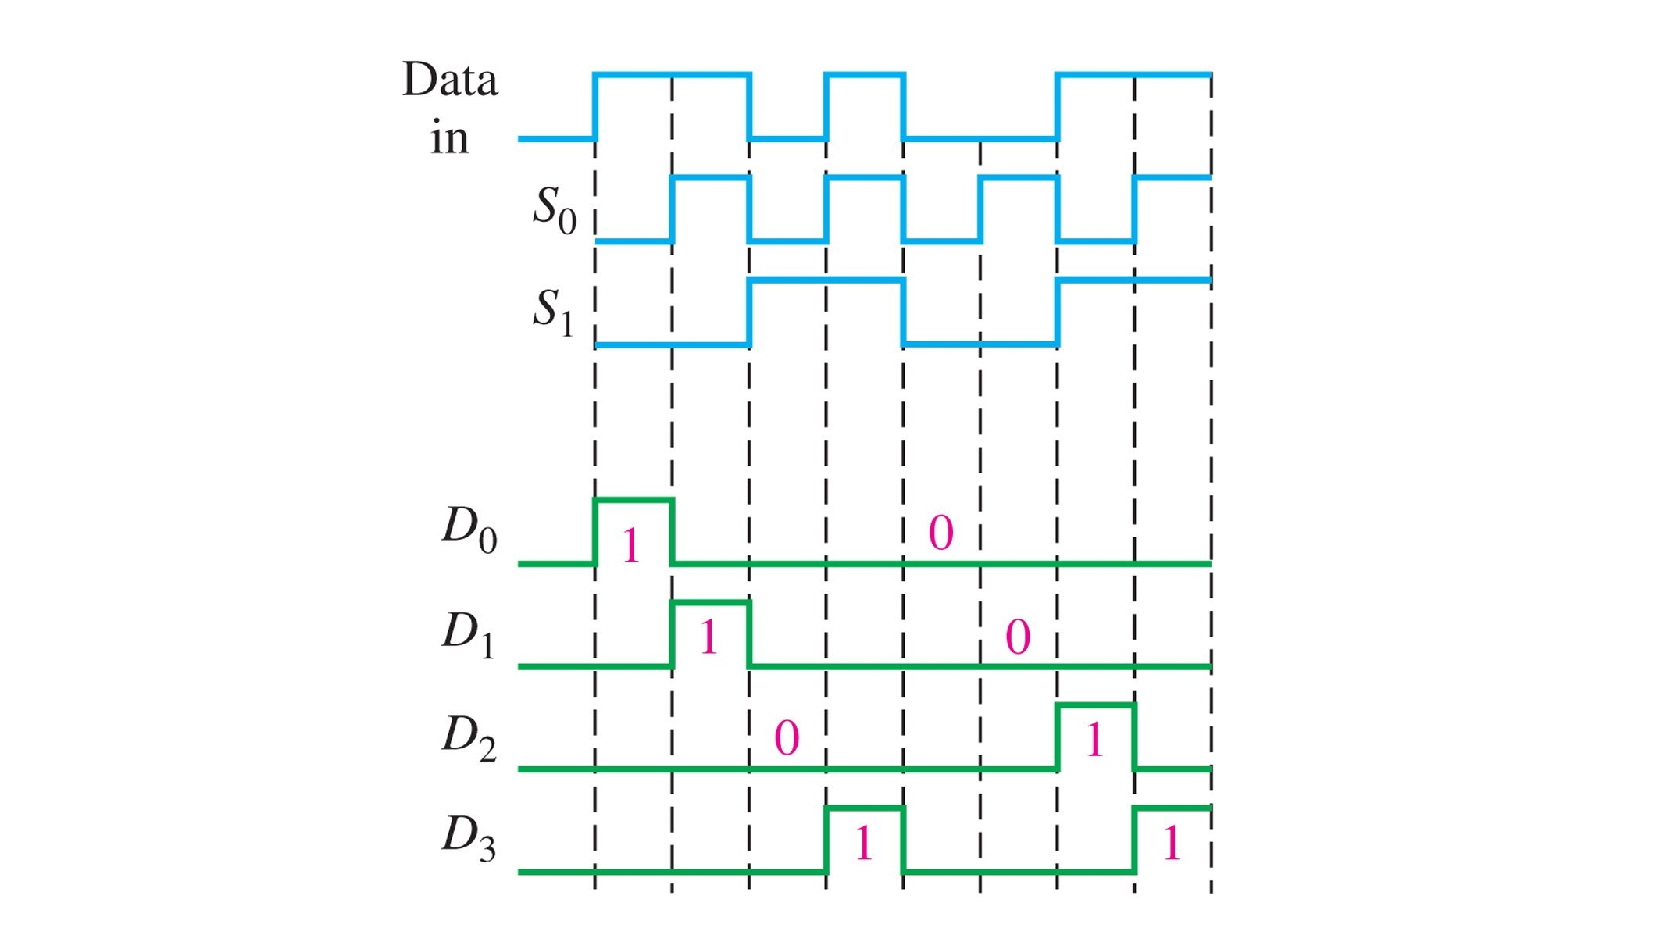
\includegraphics[width=0.75\textwidth,trim=3cm 0cm 3cm 0cm,clip=true]{figures/dmux2.pdf}
\caption{\label{fig:dmux2} One data line in and four data lines out.  \textit{Note the cadence:} we cannot know what $D_1$ is until we know what $D_0$ is...}
\end{figure}
\end{frame}

\begin{frame}{Demultiplexers}
\begin{figure}
\centering
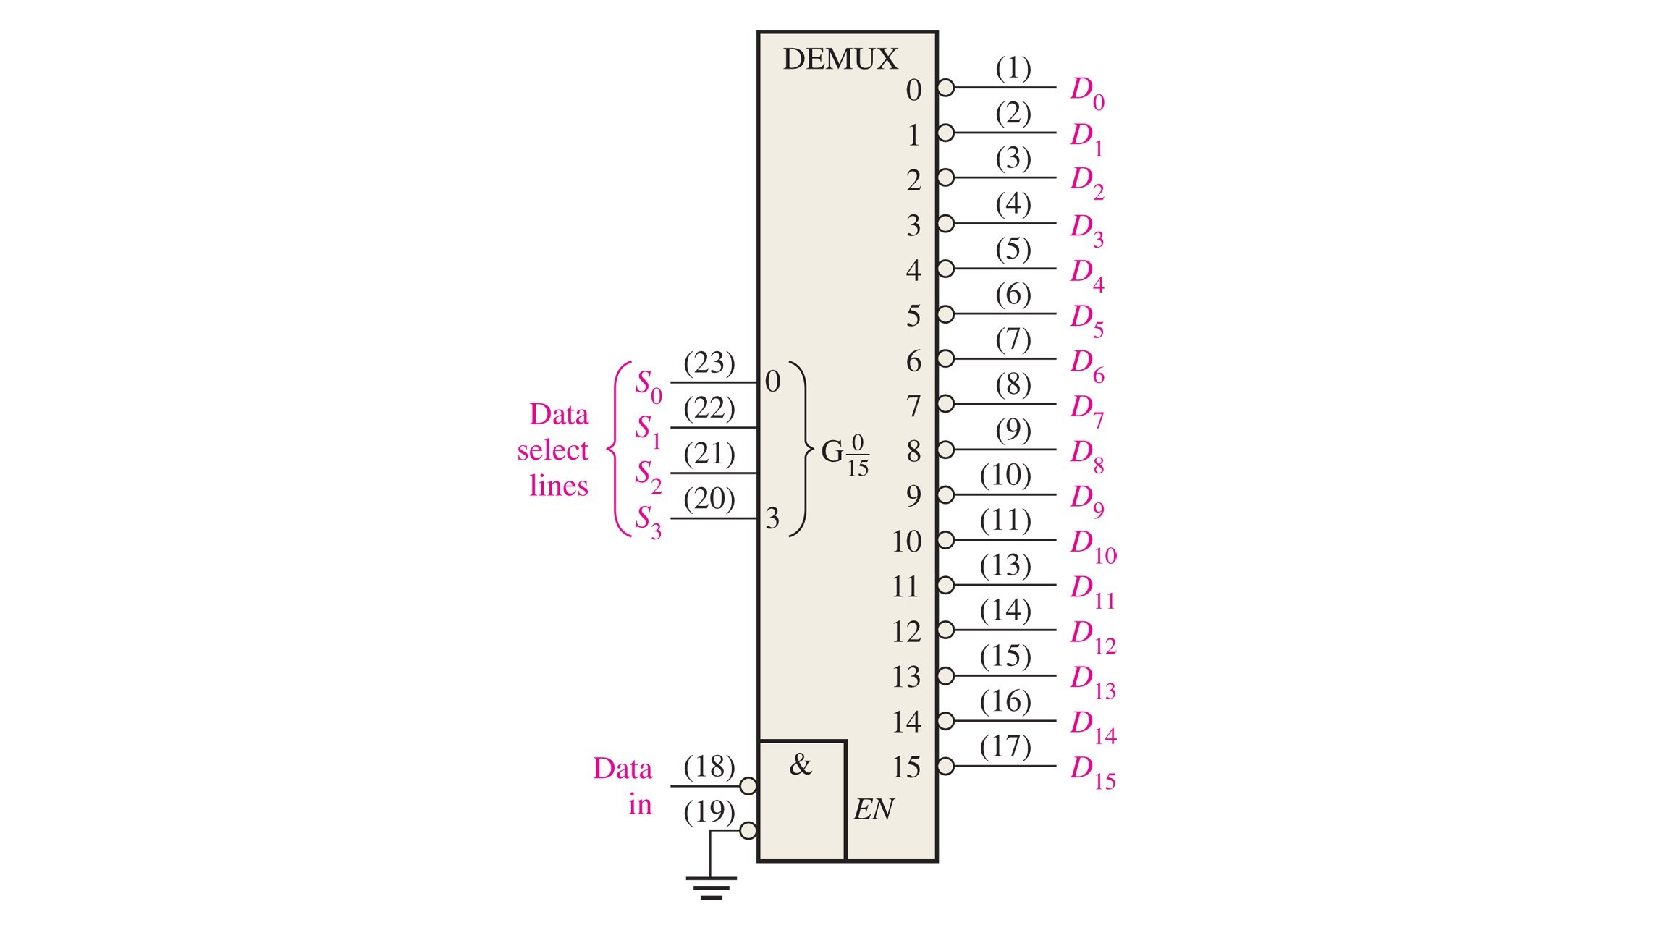
\includegraphics[width=0.75\textwidth,trim=3cm 0cm 3cm 0cm,clip=true]{figures/dmux3.pdf}
\caption{\label{fig:dmux3} A decoder is very similar to a demux, but it has to have the data input lines at the bottom left.}
\end{figure}
\end{frame}

\section{Conclusion}

\begin{frame}{Unit 3 Summary}
\alert{Functions of Combinatorial Logic} \\
\textbf{Reading:} 6-1 - 6-6 (Tuesday) \\
\textbf{Reading:} 6-7 - 6-11 (Thursday)
\begin{enumerate}
\item Half-Adders and Full-Adders
\begin{itemize}
\item Example from study guide
\item Propagation delays
\end{itemize}
\item Comparators
\begin{itemize}
\item The XNOR gate
\item Multi-bit comparators
\item Inequalities
\end{itemize}
\item Decoders/Encoders
\begin{itemize}
\item Binary to decimal circuits
\item Decimal to binary circuits
\end{itemize}
\end{enumerate}
\end{frame}

\end{document}
